\documentclass[12pt,letterpaper]{report}
\usepackage{ragged2e}
\usepackage{natbib}
\usepackage{geometry}
\usepackage{fancyhdr}
\usepackage{afterpage}
\usepackage{graphicx}
\usepackage{amsmath,amssymb,amsbsy}
\usepackage{dcolumn,array}
\usepackage{tocloft}
\usepackage{asudis}
\usepackage[pageanchor=true,plainpages=false,pdfpagelabels,bookmarks,bookmarksnumbered,hidelinks]{hyperref}

\usepackage{amssymb,amsmath}
\usepackage{amsthm}

% \biboptions{}

% The \cite command functions as follows:
%   \citet{key} ==>>                Jones et al. (1990)
%   \citet*{key} ==>>               Jones, Baker, and Smith (1990)
%   \citep{key} ==>>                (Jones et al., 1990)
%   \citep*{key} ==>>               (Jones, Baker, and Smith, 1990)
%   \citep[chap. 2]{key} ==>>       (Jones et al., 1990, chap. 2)
%   \citep[e.g.][]{key} ==>>        (e.g. Jones et al., 1990)
%   \citep[e.g.][p. 32]{key} ==>>   (e.g. Jones et al., p. 32)
%   \citeauthor{key} ==>>           Jones et al.
%   \citeauthor*{key} ==>>          Jones, Baker, and Smith
%   \citeyear{key} ==>>             1990


\usepackage{epsfig}
\usepackage{epsf}
\usepackage{psfrag}
\usepackage{caption}
\usepackage{latexsym, graphics, psfrag, amscd, amssymb, pb-diagram}

%\usepackage{algorithm}
%\usepackage{algorithmic}
\usepackage{color}
\usepackage[all,cmtip]{xy}

\usepackage[lined, ruled, linesnumbered]{algorithm2e}
\usepackage{changepage}

\newtheorem{definition}{Definition}
\newtheorem{Algorithm}{Algorithm}
\newtheorem{proposition}{Proposition}
\newtheorem{theorem}{Theorem}[section]

\usepackage{tabularx ,booktabs,wrapfig,lipsum,ragged2e}
\usepackage{multirow}
\newcolumntype{P}[1]{>{\centering\arraybackslash}p{#1}}

\newcommand{\ra}[1]{\renewcommand{\arraystretch}{#1}}


\newcommand{\myvec}[1]%
{\stackrel{\raisebox{-2pt}[0pt][0pt]{\small$\rightharpoonup$}}{#1}}
\newcommand{\Eq}[1]   {Eq.\ \ref{eqn:#1}}
\newcommand{\Eqs}     {Eqs.\ }
\newcommand{\Fig}[1]  {Fig. \ref{fig:#1}}
\newcommand{\Figs}[1] {Figs. \ref{fig:#1}}
\newcommand{\Tbl}[1]  {Table \ref{tbl:#1}}
\newcommand{\Sec}[1]  {Section \ref{sec:#1}}
\newcommand{\Secs}[1] {Sections \ref{sec:#1}}
\newcommand{\Etal}    {{\it et al}.}
\newcommand{\trans}   {\psi}
\newcommand{\acc}[1]     {$ #1 \% $}
\newcommand{\Alzheimers} {{Alzheimer\textquoteright s} }
\newcommand{\Hotellings} {{Hotelling\textquoteright s} }
\newcommand{\F}   {$ \text{F}_1 $}
\newcommand{\FDGPET}   {$ ^{18}\text{F-FDG PET} $}
\newcommand{\apoe}[1]   {Apoe$ E $#1}


\begin{document}
\sffamily
%-----------------------front matter
\pagenumbering{roman}
\title{\large{{3D - Patch Based Machine Learning Systems for Alzheimer's Disease classification via \FDGPET ~Analysis}}}
\author{Anant Srivastava}
\degreeName{Master of Science}
\paperType{Thesis}
\defensemonth{April}
\defenseyear{2017}
\gradmonth{May}
\gradyear{2017}
\chair{Dr. Yalin Wang}
\memberOne{Dr. Ajay Bansal}
\memberTwo{Dr. Jianming Liang}


\maketitle
\doublespace
\begin{abstract}

Alzheimer's disease (AD), is a chronic neurodegenerative disease that usually starts slowly and gets worse over time. It is the cause of 60\% to 70\% of cases of dementia. There is growing interest in identifying brain image biomarkers that help evaluate AD risk pre-symptomatically. High-dimensional non-linear pattern classification methods have been applied to structural magnetic resonance images (MRI's) and used to discriminate between clinical groups in Alzheimer’s progression. 
Using Fluorodeoxyglucose (FDG) positron emission tomography (PET) as the preferred imaging modality, this thesis develops two independent machine learning based patch analysis methods and uses them to perform six binary classification experiments across different (AD) diagnostic categories. Specifically, features were extracted and learned using dimensionality reduction and dictionary learning \& sparse coding by taking overlapping patches in and around the cerebral cortex and using them as features. Using AdaBoost as the preferred choice of classifier both methods try to utilize \FDGPET~as a biological marker in the early diagnosis of \Alzheimers. Additional we investigate the involvement of rich demographic features (\apoe{3}, \apoe{4} and Functional Activities Questionnaires (FAQ)) in classification. The experimental results on Alzheimer's Disease Neuroimaging initiative (ADNI) dataset demonstrate the effectiveness of both the proposed systems. The use of \FDGPET~may offer a new sensitive biomarker and enrich the brain imaging analysis toolset for studying the diagnosis and prognosis of AD.
 
{\bf Keywords:} Alzheimer’s disease, dimensionality reduction, dictionary learning and sparse coding, Patch Analysis based
Sparse-coding System.


\end{abstract}

\dedicationpage{ I am grateful to my parents for their support and encouragement.\\
	To my chair and advisor Prof. Yalin for his patience and belief in me.\\
	To my friends in Tempe for providing a healthy atmosphere.\\
	To my brother for his compassion and companionship all these years.\\
	And finally to this institution and this imprint on paper.}
\begin{acknowledgements}
	I would first like to express my gratitude to my chair, Dr. Yalin Wang, for his enthusiasm and encouragement over the years.
	I  would  also  like  to  thank  the  many  collaborators  who  have  helped  me  along  the  way,  in
	particular Liang Mi, for helping me get started and to his valuable inputs along the way, To Shibani Singh for her mathematical assistance and support, Jie Zhang, for being a mentor and to Kewei Chen and Dhruman Goradia at Banner Health for there invaluable resources and time. Thanks  also  to  all  members  of  the  Geometry Systems Laboratory group, both past and present, for providing a great working environment.
	I am also grateful to my co-chair Professor Ajay Bansal who has been a constant support and for his valuable advices and Professor Jiangming Liang for his input in my work. Finally, I am most grateful to my friends, especially everyone back in India, my family for their support and encouragement throughout my studies. Many thanks to you all.
\end{acknowledgements}

\tableofcontents
% This puts the word "Page" right justified above everything else.
\addtocontents{toc}{~\hfill Page\par}
% Asking LaTeX for a new page here guarantees that the LOF is on a separate page
% after the TOC ends.
\newpage
% Making the LOT and LOF "parts" rather than chapters gets them indented at
% level -1 according to the chart: top of page 4 of the document at
% ftp://tug.ctan.org/pub/tex-archive/macros/latex/contrib/tocloft/tocloft.pdf
\addcontentsline{toc}{part}{LIST OF TABLES}
\renewcommand{\cftlabel}{Table}
\listoftables
% This gets the headers for the LOT right on the first page.  Subsequent pages
% are handled by the fancyhdr code in the asudis.sty file.
\addtocontents{lot}{Table~\hfill Page \par}
\newpage
\addcontentsline{toc}{part}{LIST OF FIGURES}
\addtocontents{toc}{CHAPTER \par}
\renewcommand{\cftlabel}{Figure}
% This gets the headers for the LOF right on the first page.  Subsequent pages
% are handled by the fancyhdr code in the asudis.sty file.
\addtocontents{lof}{Figure~\hfill Page \par}
\listoffigures
%-----------------------body
\doublespace
\pagenumbering{arabic}
\chapter{Introduction}

Alzheimer’s disease (AD) is a chronic neurodegenerative disease in which amyloid plaques and neurofibrillary tangles accumulate in the brain. The most common early symptom is the difficulty remembering recent events (short-term memory loss). As the disease advances, patients may lack motivation, have problems with self-care, and show behavioral abnormalities or even withdraw from family and society~\citep{Burns:2009}. AD has a typical pattern of progression, with changes in the brain that correspond to the types and severity of symptoms. Disease progression has commonly been divided into five main categories in the ADNI2 phase of Alzheimer's Disease Neuroimaging initiative(ADNI)~\citep{weiner2013alzheimer}: Cognitively Normal (CN), Significant Memory Concern(SMC), Early Mild Cognitive Impairment (EMCI), Impairment (LMCI) and Alzheimer's Disease (AD), defined clinically based on behavioral and cognitive assessment. (SMC) are self-report significant memory concern from the patient we choose to exclude it from our study. Table.~\ref{fig:participant_stages} shows the participant stages across ADNI 1/2/GO.

There has been a shift with a sense of urgency to find effective intervention in the presymptomatic stage of AD so to reduce the risk of AD, delay or even prevent its onset. To more adequately diagnose different stages of the disease and especially in the early stage and predict future cognitive decline, computer-aided diagnostic classification is increasingly needed using biomarkers based on neuroimaging and other measurements.
There is evidence that the pathogenic cascade of AD is thought to begin at least 1-2 decades prior to cognitive impairment, starting with accumulation of the amyloid-$\beta$1-42(A$\beta$1-42) plaques \citep{langbaum2013ushering}. Research has suggested that these early processes can be assessed using brain imaging and fluid biomarkers. Prior research work on Fluorodeoxyglucose (FDG) positron emission tomography (PET), Pittsburgh compound B (PIB), structural magnetic resonance imaging (sMRI) and functional measures of resting-state networks (rs-fMRI) has supported their validity as potential metabolic biomarkers. Among various neuroimaging techniques, FDG-PET characterizes the cerebral glucose hypometabolism related to AD and those at risk of AD. FDG-PET offers a reliable metabolic biomarker even at pre-symptomatic stages. Despite major advances in FDG-PET used to track symptomatic patients, there is still a lack of sensitive, reliable, and accessible FDG-PET imaging algorithms capable of characterizing abnormal degrees of age-related metabolism decline in preclinical individuals at high risk for AD whom early intervention is most needed. Fig.~\ref{fig:pet_raw} shows the different types of PET scans.

Recently minor cognitive impairment (MCI) in \FDGPET ~has been classified by a brain regional sensitivity mapping method based on summated index (Total Z score) by utilizing the sensitivity-distribution maps~\citep{kakimoto2011new}.In other contemporary works a region of interest (ROI) mask is used to extract features and use incomplete random forest-robust support vector machine to perform classification~\citep{lu2017early}. In general for a classification algorithm based on 3D FDG-PET images the feature dimension is usually much larger than the number of subjects. Data with extremely high dimensionality has presented serious challenges to existing learning methods~\citep{liu2007computational}~\citep{friedman2001elements}. With the presence of a large number of features, a learning model tends to overfit, affecting its performance.

In this context, when we apply three-dimensional statistical maps to do classification the feature dimension is usually much larger than the number of subjects, i.e., the so-called “high dimension, small sample size problem”. When a vast number of variables are measured from a small number of subjects, it is often necessary to reduce their high dimension features to low dimension features. In most cases, the information gets lost by mapping into a lower-dimensional space. However, the discarding information is always compensated by a more accurate space (or feature). There are two general approaches to performing dimensionality reduction: feature selection and feature extraction. Feature selection reduces the feature dimension by selecting a subset of original variables~\citep{jain1997feature}. It aims to choose a small subset of the relevant features from the original ones according to certain relevance evaluation criterion, which usually leads to better learning performance for example higher learning accuracy for classification, lower computational cost, and better model interoperability \citep{tang2014feature}. Feature extraction reduces the dimension based on mathematical projections, which transform the original features into a lower dimensional but more appropriate feature space~\citep{guyon2008feature}. There are some widely used algorithms in machine learning, e.g., principle component analysis (PCA)~\citep{jolliffe2002principal}, linear discriminant analysis (LDA)~\citep{mika1999fisher}, as analytic tools for feature extraction.

Both Feature extraction and feature selection are capable of improving learning performance, lowering computational complexity, building better generalizable models, and decreasing required storage. Feature extraction maps the original feature space to a new feature space with lower dimensions by combining the original feature space. It is difficult to link the features from original feature space to new features. Therefore further analysis of new features is problematic since there is no physical meaning for the transformed features obtained from feature extraction techniques. While feature selection selects a subset of features from the original feature set without any transformation, and maintains the physical meanings of the original features. In this sense, feature selection is superior in terms of better readability and interpretability. This property has its significance in many practical applications such as finding relevant genes to a specific disease and building a sentiment lexicon for sentiment analysis. Typically feature selection and feature extraction are presented separately. Via sparse learning such as $\ell1$ regularization, feature extraction (transformation) methods can be converted into feature selection methods~\citep{masaeli2010transformation}. In order to analyze images more efficiently, a dictionary that allows us to represent them as a superposition of a small number of its elements so that we can reduce each image to a small number of its coefficients~\citep{schnass2008dictionary}. Similarly sparse coding \citep{lin2014stochastic} has been proposed to use a small number of basis vectors (also called dictionary) to represent local features effectively and concisely and help image content recognition. From the input image data, sparse coding learns an over-complete set of basis vectors (dictionary), which have been used to select the most germane features~\citep*{friedman2001elements}. To learn local imaging features, image patches are usually selected to form dictionaries. Dictionary learning and sparse coding \citep{mairal2009online} has shown to be efficient for many tasks such as image deblurring~\citep{yin2008bregman}, image super-resolution~\citep{yin2008bregman} functional connectivity analysis~\cite{lv2015holistic,lv2015modeling}, and image classification (Mairal et al., 2009; Moody et al., 2012). In many computer vision, medical imaging and bioinformatics applications~\citep{mairal2009online,moody2012unsupervised,lv2015modeling} dictionary learning and sparse coding leads to state-of-the-art results.

To address the problem of ``curse of dimensionality'', we propose two sets of approaches for classification of a large set of \FDGPET images, and compare their performance. The first approach consists of a learning based system with sparse coding and dictionary learning for efficient data representation (Feature Learning), maxpooling~\citep{boureau2010theoretical} for feature and again AdaBoost~\citep{rojas2009adaboost} for classification. The second approach is a empirical machine learning based model which includes patch based feature selection then maxpooling~\citep{boureau2010theoretical} for feature agglomeration. We then form data vectors and apply probabilistic principle component analysis for feature extraction using dimension reduction and finally AdaBoost for classification. The two systems serves as a comparison between the approaches for analyzing \FDGPET. Our goal is to discover an appropriate \FDGPET ~diagnosis system design by investigating their performance. We tested our hypothesis on the ADNI2 dataset across $668$ subjects. We then carried out 10 fold cross validation in six different classification experiments comparing the two methods across various imaging measures.

\begin{figure}[h]
	\centering
	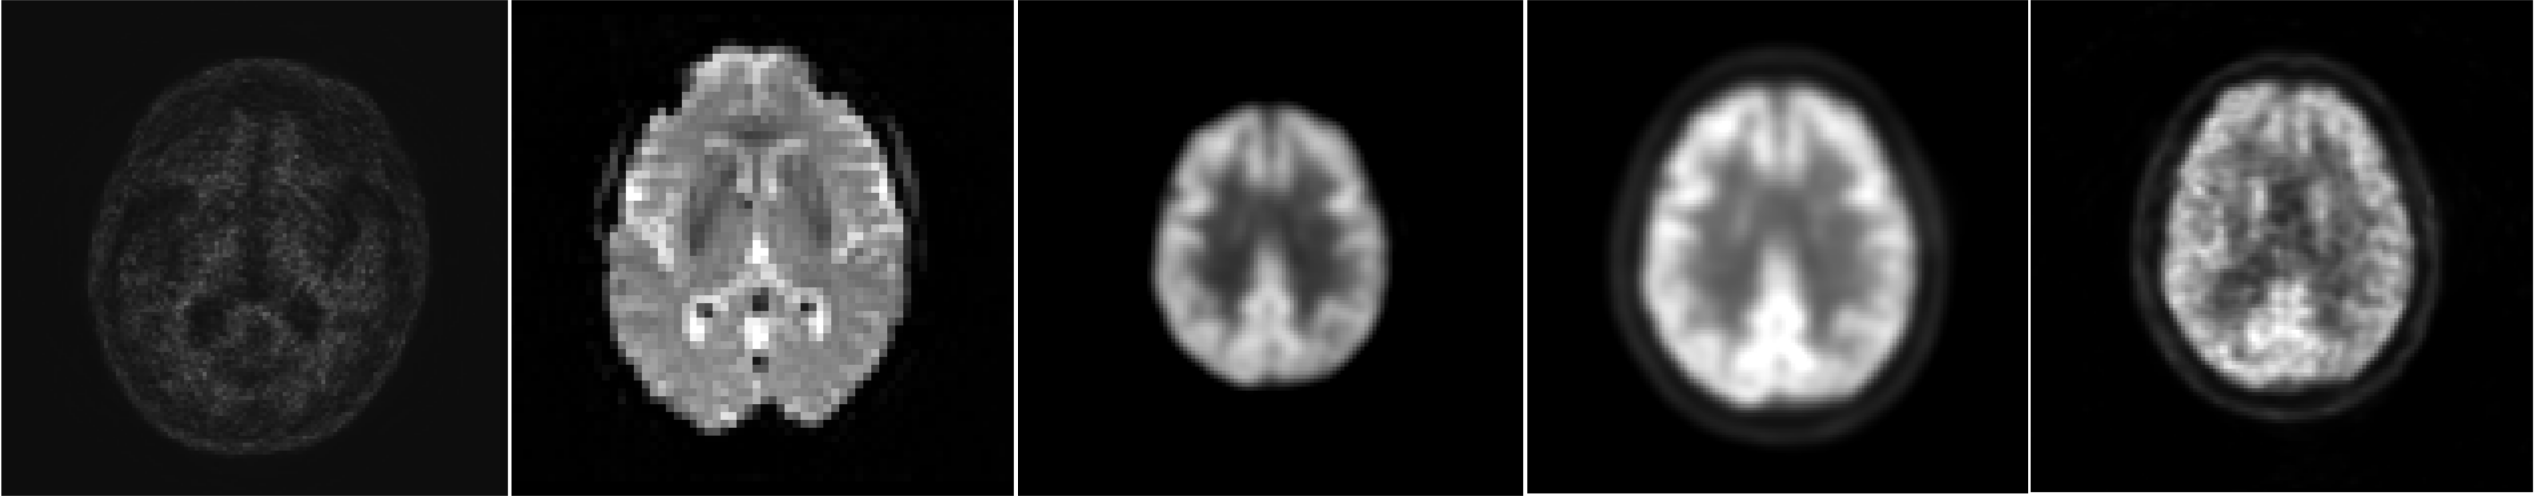
\includegraphics[width=\linewidth]{figures/pet_raw.png}
	\caption{Different types of P.E.T scans}
	\label{fig:pet_raw}
\end{figure}

{\bf Structure of document} This thesis document is divided logically into the following sections:

\begin{itemize}
	\item Chapter 2 introduces the data used in the preparation of this document and preprocessing of \FDGPET~.
	\item Chapter 3 discusses the background and history of both our proposed methods. It also discuses the role of \FDGPET~as a biomarker. A brief history of the techniques used and motivation. The techniques used are introduced. 
	\item Chapter 4 discusses the system design and architecture in detail and addresses the major components of the system.	
	\item Chapter 5 describes the experimental setup, presents the results and sheds light on the tools analysis. We show the result of classification in both methods. We compare and perform meta-analysis on stochastic coordinate coding (SCC) and dimensionality reduction (feature extraction) and investigate addition of other features. 
	\item Chapter 6 continues our discussion on the results, lessons learned over the course of the project, the limitations and talk about the further improvements.
	\item Chapter 8 concludes the thesis, with ideas about future works.
	
\end{itemize}
	
In this work we shed some light on \FDGPET~as a biomarker and we try to evaluate our statistical map to find a better diagnosis of (AD). In summary we make the following contribution.

\begin{itemize}
	\item We use the second phase of ADNI as our choice of dataset. It is relatively new and has extensive subject information.
	\item Building two empirical series of Machine Learning systems on the above dataset and check the performance of state-of-the art algorithms on \FDGPET.
	\item Introduction of a few demographic features in the classification process which drastically improves performance.     
\end{itemize}    	
	

\chapter{Subjects and Data Preprocessing}
\label{chapter:subjects_perprocessing}
This chapter focuses on ADNI and its study phase ADNI2. The first section briefly describes the history and background of ADNI and our choice of data acquisition   

\section{Subjects}
\label{sec:subjects}
Data used in the preparation of this article were obtained from the Alzheimer\textquoteright s Disease Neuroimaging Initiative (ADNI) database (adni.loni.usc.edu). The ADNI was launched in 2004 by the National Institute on Aging (NIA), the National Institute of Biomedical Imaging and Bioengineering (NIBIB), the Food and Drug Administration (FDA), private pharmaceutical companies and non-profit organizations, as a \$60 million, 5-year public private partnership. The primary goal of ADNI has been to test whether serial magnetic resonance imaging (MRI), positron emission tomography (PET), other biological markers, and clinical and neuropsychological assessment can be combined to measure the progression of mild cognitive impairment (MCI) and early Alzheimer\textquoteright s disease (AD). Determination of sensitive and specific markers of very early AD progression is intended to aid researchers and clinicians to develop new treatments and monitor their effectiveness, as well as lessen the time and cost of clinical trials.

ADNI is the result of efforts of many coinvestigators from a broad range of academic institutions and private corporations, and subjects have been recruited from over 50 sites across the U.S. and Canada. The initial goal of ADNI was to recruit 800 subjects but ADNI has been followed by ADNI-GO and ADNI-2. To date, these three protocols have recruited over 1500 adults, ages 55 to 90, to participate in the research, consisting of cognitively normal older individuals, people with early or late MCI, and people with early AD. The follow up duration of each group is specified in the protocols for the three phases if ADNI: ADNI-1, ADNI-2 and ADNI-GO. Subjects originally recruited for ADNI-1 and ADNI-GO had the option to be followed in ADNI-2. For up-to-date information, see www.adni-info.org.

Although the three studies all aim to advance AD research, there is some differences in participant pools, and adjustments to data collection protocols over time as a result of scientific findings and changing technologies. ADNI2 phase started in January 2011 and ended January 2016. ADNI1 has been a topic of research in our laboratory~\citep{shi2014genetic,zhang2016morphometric} and this motivated us to analyze ADNI2. Participants were recruited across North America during each phase of the study and agreed to complete a variety of clinical assessments. The studies includes participants to make multiple visits but in this study we refrain to baseline and screening data, the marked region in Fig.~\ref{fig:study_schedule}.

\begin{figure}
	\centering
	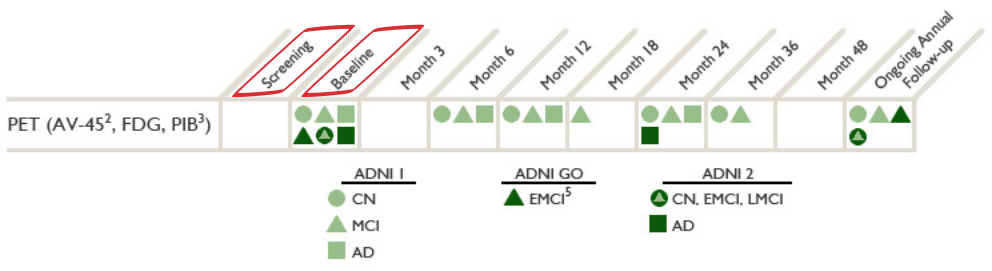
\includegraphics[width=\linewidth]{figures/Imaging_Chart_PET.png}
	\caption[Summary of Clinical Data]{The summary of the clinical data for FDG-PET scans ADNI1 is indicated ny light green and the later phases ADNI 2 \& GO are represented by dark green. The typical timeline for image accusation is over 4-5 years and the initial phase is Screening and Baselines. Given the consistency of data for ADNI2 at Baseline we choose the latter for analysis.}
	\label{fig:study_schedule}
\end{figure}
 

\begin{table}
	\centering
	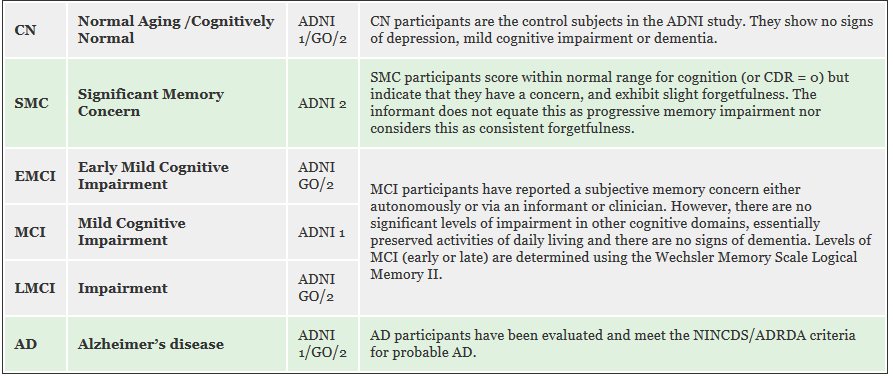
\includegraphics[width=\linewidth]{figures/participant_stages.png}
	\caption[Participant Stages across ADNI 1/GO/2.]{Participant Stages across ADNI 1/GO/2.\footnote{http://adni.loni.usc.edu/study-design/background-rationale/}}
	\label{fig:participant_stages}
\end{table}
  
For this thesis, we studied a total of 668 subjects in the ADNI2 baseline dataset, within this population, there were 146 who had \Alzheimers (AD), 158 had impairment (LMCI), 178 had early mild cognitive impairment (EMCI) and 186 were normal control (CN). Table.~\ref{fig:participant_stages} gives a detailed description of all the stages in disease progression. (SMC) is a new cohort in ADNI 2, it is introduced in the study to minimize the stratification risk among normal control and addressing the gap between healthy elderly controls and Impaired. We choose to ignore (SMC) from our study as the participants with (SMC) suffer from slight forgetfulness and they have a cognitive dementia rating (CDR)~\citep{morris1993clinical} of zero and thus is very loosely based to clinical dementia. 

\section{Data Gathering}
\label{sec:data_gathering}
To acquire \FDGPET data from the ADNI LONI website one has to complete an application process which includes the acceptance of a data user agreement and the submission of and online application form. It is also required that the application includes the institutional affiliation and the proposed research to be conducted using the ADNI data. The image collections are downloaded from the ADNI LONI database at (https://ida.loni.usc.edu). We initially download the image scans across all the accusation stages from the image search engine. We select the uniform pre and post processed scans and download the data in ``NiFTI'' format. Out of $1340$ subjects $774$ were present at baseline and were used in our experimentation.
\begin{figure}[h]
	\centering
	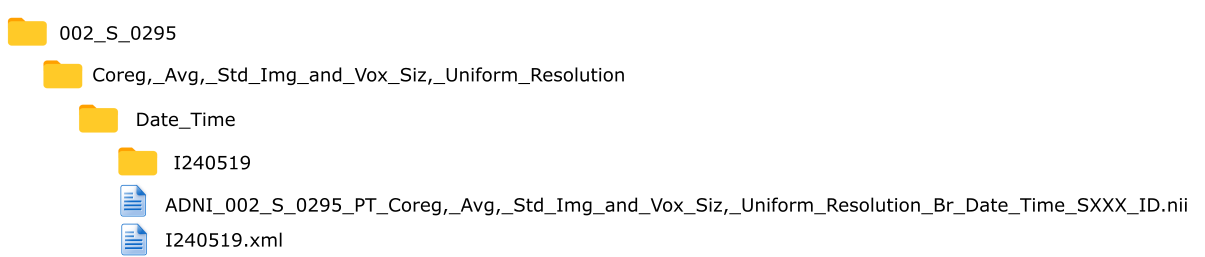
\includegraphics[width=\linewidth]{figures/file_structure}
	\caption[The File Structure of a Participant]{The File Structure of a Participant.}
	\label{fig:filestructure}
\end{figure}

\begin{table}[t]
	\begin{center}
		\caption{Demographic Information of $668$ Subjects in the ADNI2 Baseline Dataset.}\label{tab:demographic}
		\begin{tabular}{|P{1.5cm}|P{1cm}P{1cm}P{2.25cm}P{3cm}P{1.25cm}P{1.25cm}P{1.25cm}|}
			\hline
			& Male & Female & Age & Min~/~Max Age & APOE1 & APOE2 & FAQ \\
			\hline\hline
			AD 		& $85$ 	& $61$ & $74.73 \pm 8.15$ 	& $56~/~90$ &	3.11 & 3.63 & 13.39\\
			LMCI 	& $84$ 	& $74$ & $72.5 	\pm 7.5$ 	& $55~/~91$ &	3.03 & 3.54 & 03.62\\
			EMCI 	& $102$ & $76$ & $ 71.3 \pm 7.2 $	& $55~/~89$ &	2.94 & 3.42 & 02.08\\
			CN 		& $89$ 	& $97$ & $ 73.5 \pm 6.25 $ 	& $57~/~89$ &	2.86 & 3.24 & 00.16\\
			\hline
		\end{tabular}
	\end{center}
\end{table}

Fig.~\ref{fig:filestructure} shows the file structure of one participant in the downloaded image collection. Participant is given a subject ID: ``002\_S\_0295'' as shown in Fig~\ref{fig:filestructure}. In the ADNI study after image accusation the \FDGPET ~scans are filtered with a scanner-specific filter function to produce images of a uniform isotropic resolution of 8 mm FWHM. These preprocessed PET data are co-registered, averaged image from their baseline PET scans, which are then reoriented into a standard $160\times160\times96$ voxel image grid, having 1.5 mm cubic voxels. This image grid is oriented such that the anterior-posterior axis of the subject is parallel to the AC-PC line \citep{lee2014parametric}. This standardized image then serves as a reference image for all PET scans on that subject. Fig.~\ref{fig:filestructure} shows the folder name ``Coreg,\_Avg,\_Std\_Img\_and\_Vox\_Siz,\_Uniform\_Resolution'' indicating the type of preprocessing. Additionally a subject may have participated only at the baseline accusation and some other subject may have been involved at both baseline and ADNI-1 year, so a patient may have more than one scan of which we only investigate the baseline one. In Fig~\ref{fig:filestructure} folder ``Date-Time'' has only one record indicating the presence of only one Baseline scan.

Each scan has a unique ID (``I240519'' in Fig.~\ref{fig:filestructure}) and associated to it is a XML file. Form this structure we extract all the XMLs and the NiFTI image scans. To learn about the demographics and segregate the stages in (AD) disease progression we use python to crawl over the XML files. We extract key demographic information from the XMLs and make a dictionary segregating the baseline scans from other visits. From this we form six sets of collections over which we will run our proposed methods. Table.~\ref{tab:demographic} shows the demographic information of the participants.  


\section{Image Preproceessing}
\label{sec:image_preprocessing}
For a patch based method to work on 3D images it requires that a significant portion of the cerebral \FDGPET ~image scan is represented by the generated patches. To minimize the empty and non-essential space in and around the relevant region of interest (ROI), further processing is essential. Fig.~\ref{fig:preprocessing}(a.) shows the data that we immediately get after downloading the \FDGPET ~image scans, as seen in Fig.~\ref{fig:preprocessing}(a.) the scan is surrounded by empty voxels which convey no information and we wish to get rid of it. Before we crop the 3D-image scans we will have to spatially normalize Fig.~\ref{fig:preprocessing}(b.) the image to bring all the scans to a same space. Human brain differs in size and shape and thus goal of spatial normalization is to deform the human brain scans so one subject's brain scans corresponds the same location in another subject's brain scans. To refrain ourself in using only the cerebral ROI we further segmented the scans. Fig.~\ref{fig:preprocessing}(c.) is the normalized and segmented version of our data. 
\begin{figure}[h]
	\centering
	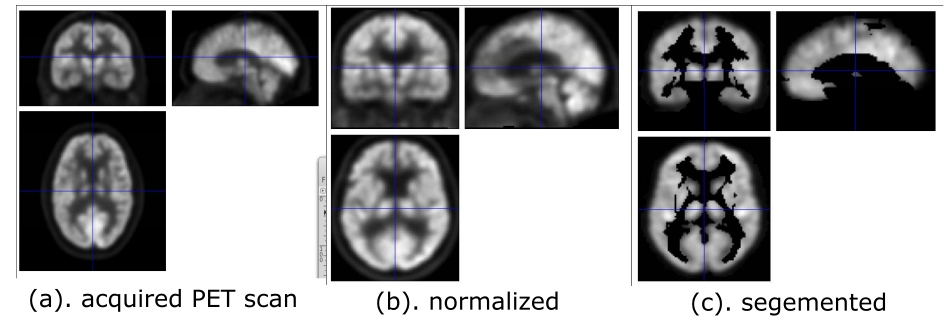
\includegraphics[width=\linewidth]{figures/preprocessing}
	\caption[Prepocessing Pipeline]{Preprocessing Pipeline in FDG-PET. (a.) accuired data (b.) aligned \& normalized (c).skull stripped and segemented.}
	\label{fig:preprocessing}
\end{figure}
    
Given a FDG-PET image, the alignment and the image segmentation are automatically performed  software toolkit Statistical Parametric Mapping (SPM12)~\citep{penny2011statistical}\footnote{http://www.fil.ion.ucl.ac.uk/spm/}. Firstly to linearly align all the images into a common space and normalize them we use the (SPM) batch editor. As indicated in Fig~\ref{fig:filestructure} the baseline scans of all the subjects are unique by the image-UID (e.g. ``I240519'') and we can easily mark and distinguish files by this ID. Keeping this in mind we batch normalize and rename the NiFTI files as ``ImageUID.nii'', below is a portion of the .m file created and loaded in to the batch editor for normalization. 
\begin{figure}[h]
	\centering
	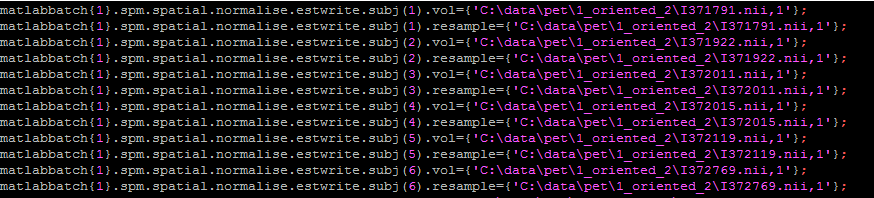
\includegraphics[width=\linewidth]{figures/batching}
	\caption[Code Snippet for Batching Data into SPM]{Code snippet for batching data into spm}
	\label{fig:batching}
\end{figure}

Second, we borrow a brain mask from SPM, an AAL template to decide which regions to keep and which to remove. We align the template to the same space as we did to the test images and turn the AAL template (Fig.~\ref{fig:mask}) into a mask by turning all the non-zero voxels to the value of ``1''. Third we compute the dot product of the FDG-PET image scans and the mask generated to segment the region of interest. Keeping the nomenclature of the files consistent with the previous step. Fourth, we conduct spatial smoothing with a Gaussian kernel of the full width at half maximum (FWHM) equal to (8; 8; 8) in three directions (x; y; z).
\begin{figure}[h]
	\centering
	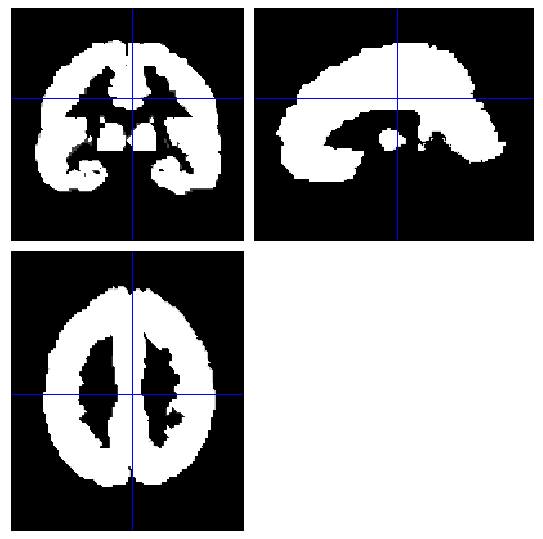
\includegraphics[width=\linewidth]{figures/mask}
	\caption[AAL Mask used for Segementation]{AAL mask used for segementation}
	\label{fig:mask}
\end{figure}

 

\chapter{Methods and Background}
In this chapter we formulate our problem background and the history of machine learning and PET images in literature. After setting us some goals and motivation we will introduce in brevity the Machine Learning techniques we propose to use.  

\section{Background}
\label{sec:background}
In Chapter.~\ref{chapter:subjects_perprocessing} the PET data is processed and made ready to use. In this section we look into the problem background, formulate mathematical frameworks to base our analysis and look into the history of Machine Learning with respect to \FDGPET~and discuss it as a reliable biomarker.

\subsection{Problem Background}
ADNI2 is divided into five cohorts namely (AD), (LMCI), (EMCI), (SMC) and (CN) (Table.~\ref{fig:participant_stages}). The overall goal of ADNI is to validate biomarkers for use in Alzheimer’s disease clincal treatment trials. ADNI is not a population based study and enrolls selected populations who may be used in future treatment trials. Therefore the results from ADNI may not be generalizable to other populations. Dementia, one of the most feared associates of increasing longevity, represents a pressing public health problem and major research priority. The ADNI study is a major step toward the early diagnosis and detection of (AD). Increasing knowledge over the last years about the pathomechanisms involved in AD allow for the development of specific treatment strategies aimed at slowing down or even preventing neuronal death in AD.

There is a sense of urgency in find imaging techniques and biomarkers. It is required that:

%% reason for choosing PET

\begin{itemize}
	\item AD be classified from normal control with high accuracy because non-AD dementias would not benefit from an AD-specific treatment
  	\item AD progression be tracked and distinguished from lower levels of dementia (EMCI, LMCI \& SMC in case of ADNI2) when an intervention would be most effective.
  	\item The treatment efficacy be reliably and meaningfully monitored 
\end{itemize}

In the report by \citep*{mueller2005ways} there is a mention that no one biomarker exists yet that fulfills all the above requirements. Yet there is increasing evidence that a combination of currently existing neuroimaging techniques and different biomarkers can provide important complementary information and thus contribute to a more accurate and earlier diagnosis of AD. Leading us to investigate the demographic feature.  

We design six experiments (1). AD vs. CU (2). AD vs. EMCI (3). AD vs. LMCI (4). CU vs. EMCI (5). CU vs. LMCI (6). EMCI vs. LMCI. The objective here is to independently study the inter-cohort relationships in hope of learning more about the class separation in AD clinical group.

\subsection{History of M.L. and FDG-PET}
A \FDGPET~ scan uses a small amount of fluorodeoxyglucose (FDG) tracer ergo ``FDG-PET'' to show differences between healthy tissue and diseased tissue. The radioactive tracer will take 30 to 90 minutes for it to travel through the body. In previous studies FDG-PET is described as a
“neuronal injury” biomarker in AD~\citep{ishii2002clinical,ishii2014pet}.

In the report ``PET approach for dementia diagnosis''\cite{ishii2014pet} states that FDG-PET generally has a higher accuracy than MR imaging for diagnosis of early AD and for predicting rapid conversion for mild cognitive impairment (MCI) to AD. This is corroborated by Fig.~\ref{fig:biomarker} where the strength of the curve is maximum for amyloid-PET during the early stages. For statistical voxel based analysis the researches have proposed for automatic diagnosis the t-sum method of calculating the total t-values in a region-of-interest template by using the Statistical Parametric Mapping (SPM) program. 
In other works \citep*{rabinovici2011amyloid} FDG-PET has been compared against amyloid ligand Pittsburgh
compound B (PiB-PET) and has been used to differentiate between  frontotemporal lobar degeneration (FTLD) and AD. The study concluded that PiB and FDG showed similar accuracy in discriminating AD and FTLD. 

%% edit t values and z score correction
For 3D PET scans ``Z-score'' images are used to represent the active parts of the brain it will show all pixels with values below the lower threshold in blue, and pixels above the upper threshold in red~\citep{ishii2014pet}. PET scans have also been analyzed by utilizing adjusted $T$ statistics and an automated voxel-based procedure~\citep{herholz2002discrimination} and Machine Learning algorithms to address the high dimensionality of the statistical maps~\citep{illan201118}~\citep{higdon2004comparison}. Recently minor cognitive impairment (MCI) in \FDGPET ~has been classified by a brain regional sensitivity mapping method based on summated index (Total Z score) by utilizing the sensitivity-distribution maps~\citep{kakimoto2011new}. In other contemporary works a region of interest (ROI) mask is used to extract features and use incomplete random forest-robust support vector machine to perform classification~\citep{lu2017early}. In previous work within our lab MRI images were classified using surface measures of ventricular enlargement and sparse coding then applied on the 2D-patch features~\citep*{zhang2016hyperbolic,zhang2016applying} with $ 96.7 \% $ accuracy. These images were functional MRIs and the features were a combination of surface statistics, we build our idea on a similar model we fist design a empirical machine learning based model. Using three dimensional patches (i.e., small sub volumes of the image defined as three-dimensional [3D] cubes) we extract information. A very similar 3D patch based feature selection is described in \citep{coupe2011patch}, In  this work, voxels  with  similar  surrounding  neighborhoods  are  considered  to  belong  to  the  same  structure and thus are used to estimate the final label. Our data is also along the same lines. 

\subsection{Biomarker}
The Figure~\ref{fig:biomarker} depicts the biomarkers as indicator of dementia. The curve indicates the strength of the biomarker with respect to dementia state. The common imaging and assessment modalities are:
\begin{enumerate}
	\item Amyloid beta imaging modality detected in CSF and PET-Amyloid.
	\item Neuro-degeneration detected by \FDGPET.
	\item Brain atrophy and neuron loss measured with MRI.
	\item Memory loss measured by cognitive assessment
	\item General cognitive decline measured by cognitive assessment 
\end{enumerate}

1-3 biomarkers can be observed before the diagnosis of dementia, and our data is of the second type measuring the neuronic activity at a given time. \FDGPET~ scan is a 30 min procedure and requires the patient to stay still in a dark room. The varition in neuronic activity at a time if any is accounted as outliers and it depends on the chosen algorithms to handle outliers. The graph in Fig.~\ref{fig:biomarker} gives us an insight into how out classification would perform given the biomarker as \FDGPET. AD vs. CU would be easily separable, groups like EMCI vs. LMCI who have close separation in progression may be the most difficult to classify and early changes in disease progression should have a strong separation but not as strong as in case of AD vs. CU.        

\begin{figure}[h]
	\centering
	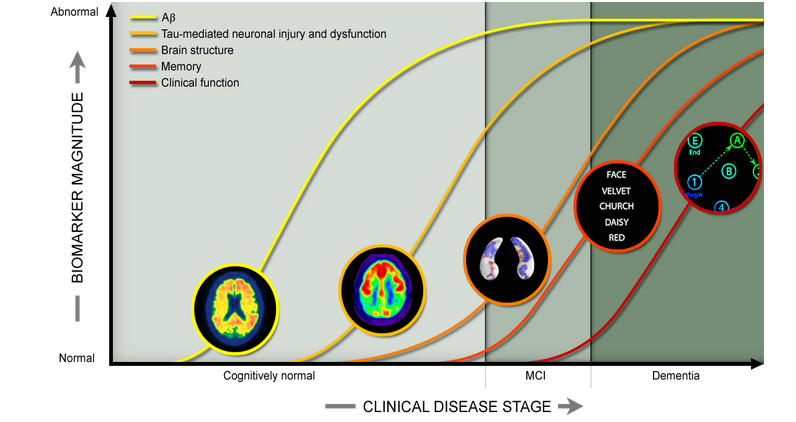
\includegraphics[width=\linewidth]{figures/biomarker}
	\caption[Biomarkers vs. Dementia]{Biomarkers vs. dementia in symptomatic stages of AD. The curves to right (yellow(PET), melon-orange (PET)) have strong early slopes indicating early class separation, curves to the right (orange (MRI), red (assessments)) have strong slopes in later stages.}
	\label{fig:biomarker}
\end{figure}


\section{Methods}
\label{sec:theoritical_background}

In this section, we briefly introduce the most relevant theoretical background in Sparse Coding, Dimensionality Reduction, Max-Pooling and Adaptive Boosting (Adaboost). The underlying algorithm are described in detail in Chapter.~\ref{chapter:algorithm}.

\subsection{Dictionary Learning and Sparse Coding} 
Sparse coding is the modeling of data vectors as sparse linear combinations of basis elements it is widely used in machine learning, neuroscience, signal processing, and statistics. From the input image data, sparse coding learns an over-complete set of basis vectors (dictionary), which have been used to represent data efficiently~\citep{tibshirani1996regression,friedman2008sparse}. To learn local imaging features, image patches are usually selected to form dictionaries. We first generate a 10 $\times$ 10 $\times$ 10 window on the 3D scan to obtain a collection of small image patch with constant overlap. We used the technique of dictionary learning and sparse coding to learn meaningful features based on stochastic approximations, which scales up gracefully to large datasets with millions of training samples. Stochastic Coordinate Coding (SCC)~\citep{lin2014stochastic} was adopted in our work for dictionary construction because of its computational efficiency.

Given a data set $\mathbf{X} = (x_1 \dots x_n)$ of image patches, each image patch is a {\em p}-dimensional vector i.e., $ x_i \in \mathbb{R}^{p} $, $ i = 1, \dots, n $. Specifically, suppose there are \emph{m} atoms $ \mathbf{d_j} \in \mathbb{R}, j = 1,\dots,m $, where the number of atoms is usually much smaller than the number of image patch {\em p}. Each patch can be represented as $ \mathbf{x_i} =  \sum^m_{j=1} z_{i,j}d_j $. In this way, the {\em p}-dimensional vector $ \mathbf{x_i} $ is represented by an m-dimensional vector $  \mathbf{z_i} = (z_{i,1},\dots,z_{1,m})^T $ which means the learned feature vector $ \mathbf{x_i} $ is a sparse vector. We can then formulate the following optimization problem:

\begin{equation}\text{min} \,\, f_i(D,z_i) = \frac{1}{2}\|Dz_i - x_i\|^2 + \lambda\|z_i\|_1 \end{equation}

where $ \lambda $ is the regularization parameter, $ \|\,.\,\| $ is the Euclidean norm and $ \|z_i \|_1 = \sum^m_{j=1}|z_{i,j}| $. We can interpret the first term of the Eq(1) as a reconstruction term which tries to force the algorithm to provide a good  representation of $\mathbf{x}$. The second term of Eq(1) ensures the sparsity of the learned features $ \mathbf{z_i} $. $ D = (d_1,\dots,d_m) \in \mathbb{R}^{p \times m} $ is the dictionary. Given the whole dataset $\mathbf{X}$., the sparse coding problem is then given as follows:
\begin{equation}\underset{D \in B_m,\mathbf{z_1},\dots,\mathbf{z_m}}{\text{min}} \,\, \mathcal{F}(D,z_1,\dots,z_m) \equiv \frac{1}{n}\sum^n_{i = 1}f_i(D,z_i),\end{equation}

It is a non convex problem with respect to joint parameters in the dictionary  $\mathbf{D}$ and the sparse code $ \mathbf{Z} = \mathbf{z_1},\dots,\mathbf{z_m} $.However, it is a convex problem when either D or Z is fixed. When the dictionary is fixed, solving each sparse code $z_i$ is a Lasso problem. Because the PET scan feature dimension $m$ is much larger than than $n$, solving the Lasso problem is time consuming. On the other hand when the sparse codes are fixed, it will become a quadratic problem. Solving the sparse coding problem also requires a lot of time when dealing with large-scale data sets and a large-size dictionary. Thus we choose the stochastic coordinate coding(SCC) algorithm~\citep{lin2014stochastic}, which can dramatically reduce the computational costs of the sparse coding while keeping a comparable performance. The dictionary learning and sparse coding based on SCC algorithm may involve many rounds of iteration. One iteration is described in Fig.~\ref{fig:iteration}. In many computer vision, medical imaging and bioinformatics applications~\citep{mairal2009online,zhang2010discriminative,lv2015modeling} dictionary learning and sparse coding leads to state-of-the-art results.
\begin{figure}[h]
	\centering
	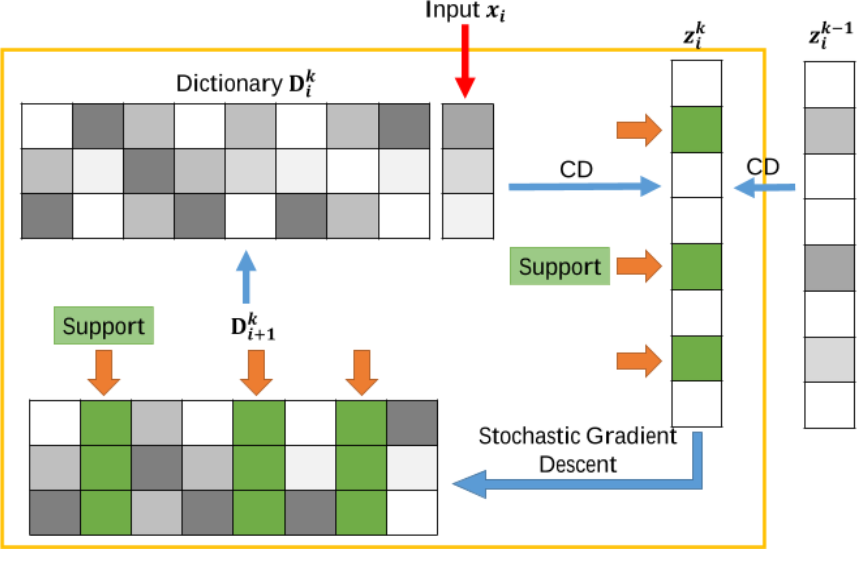
\includegraphics[width=\linewidth]{figures/iteration}
	\caption[One Iteration of SCC]{Figure shows one iteration of the sparse coding algorithm. (a).Take an image patch $x_i$. (b). Perform few steps of coordinate descent to find the support (non zero entries) of the sparse code. (c). Update the support of the dictionary by second order stochastic gradient descent to obtain a new dictionary.}
	\label{fig:iteration}
\end{figure}

\subsection{Max-Pooling} 
State-of-the-art patch-based image representations involve a pooling operation that aggregates statistics computed from local descriptors. After obtaining features using convolution, we would next like to use them for classification. In theory, one could use all the extracted features with a classifier such as a softmax classifier, but this can be computationally challenging. We use max-pooling which summarizes the coded features over larger neighborhoods. To address this, first recall that we decided to obtain convolved features because images have the "stationarity" property, which implies that features that are useful in one region are also likely to be useful for other regions. Thus, to describe a large image, one natural approach is to aggregate statistics of these features at various locations. If one chooses the pooling regions to be contiguous areas in the image and only pools features generated from the same (replicated) hidden units. Then, these pooling units will then be translation invariant. This means that the same (pooled) feature will be active even when the image undergoes (small) translations. Translation-invariant features are often desirable; in many tasks (e.g., object detection, audio recognition), the label of the example (image) is the same even when the image is translated. For example, if you were to take an MNIST digit and translate it left or right, you would want your classifier to still accurately classify it as the same digit regardless of its final position. Standard pooling operations include sum- and max-pooling. Sum-pooling lacks discriminability because the resulting representation is strongly influenced by frequent yet often uninformative descriptors, but only weakly influenced by rare yet potentially highly-informative ones. Max-pooling equalizes the influence of frequent and rare descriptors but is only applicable to representations that rely on count statistics, such as the bag-of-visual-words (BOV) and its soft-and sparse-coding extensions. Fig. \ref{fig:maxpooling} shows the whole process of max pooling. On the left hand side, pooling layer down-samples the volume spatially, independently in each depth slice of the input volume. On the right hand side, it is the most common max pooling shown with a stride of 2.
\begin{centering}
	\begin{figure}
		\centering
		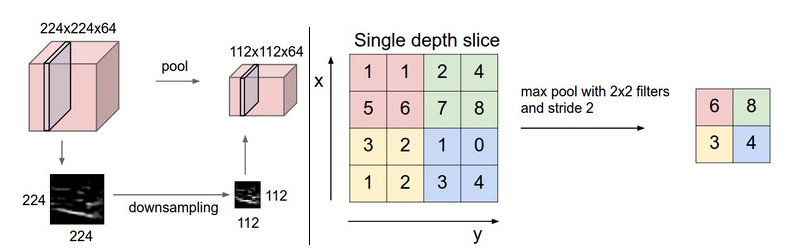
\includegraphics[width=\linewidth]{figures/maxpooling2.png}
		\caption[Maxpooling and Downsampeling.]{Pooling layer down-samples the volume spatially, independently in each depth slice of the input volume. Left: In this example, the input volume of size [$256\times256\times16$] is pooled with filter size 2; stride 2 into output volume of size [$128\times128\times16$]. Notice that the volume depth is preserved. Right: The most common down-sampling operation is max, giving rise to max-pooling, and here shown with a stride of 2, each max value is taken over 4 numbers (little $2\times2$ square).}
		\label{fig:maxpooling}
	\end{figure}
\end{centering}

\subsection{Dimension Reduction}
Feature extraction approaches project features into a new feature space with lower dimensionality and the new constructed features are usually combinations of original features. Examples of feature extraction techniques include Principle Component Analysis (PCA), Linear Discriminant Analysis (LDA) and Singular Value Decomposition(SVD). Feature extraction maps the original feature space to a new feature space with lower dimensions by combining the original feature space. In that context principle component analysis (PCA)~\citep{jolliffe2002principal} is a unsupervised machine learning algorithm widely used for dimensionality reduction. It used orthogonal transformations to convert a set of observations of possibly co-related values into a set of linearly uncorrelated variables called principle components. 

After selecting the patches and structuring our 3D data into ``sample $ \times $ features'', we would wish to analyze it summarizing its main characteristics. PCA is one of the most popular techniques for processing, compressing and visualising data. We use probabilistic PCA a variation of traditional PCA to reduce the dimensions of our selected features. Traditionally PCA's effectiveness is limited by its global linearity, to overcome that a combination of local linear PCA projections has been found to be able to capture data complexity efficiently. This model variant of PCA corresponds to the probability density unlike traditional PCA and enables it to combine PCA models~ \citep{tipping1999mixtures}. After reducing the dimensions of our dataset we will classify using AdaBoost. 


\begin{centering}
	\begin{figure}
		\centering
		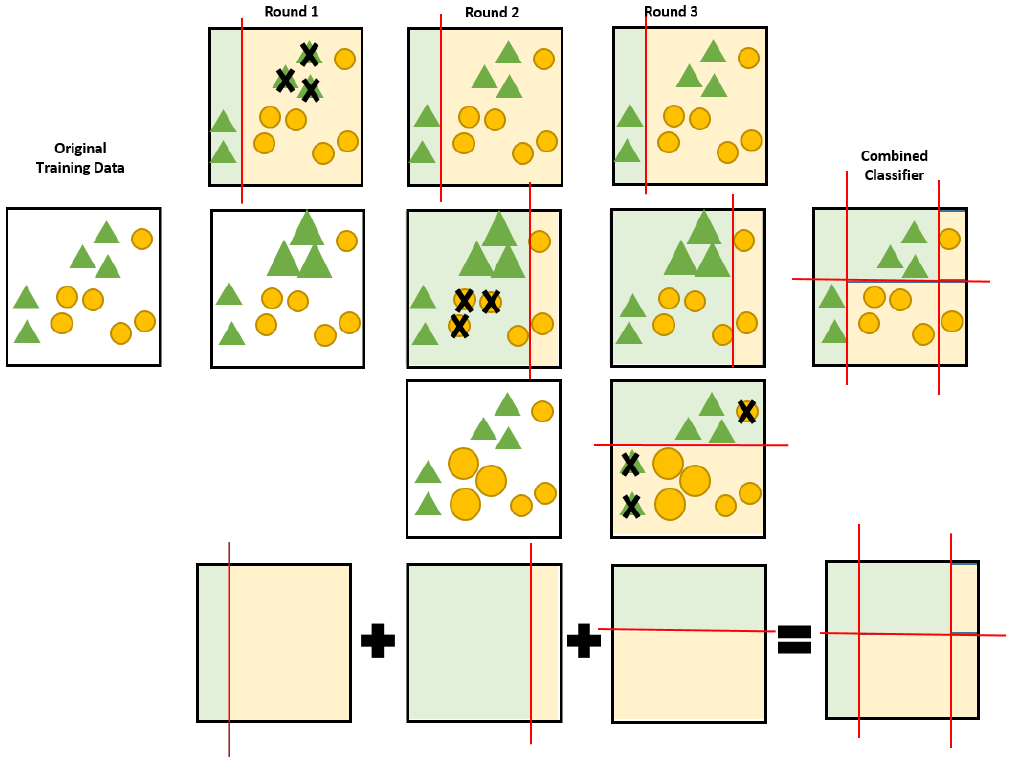
\includegraphics[width=\linewidth]{figures/adaboost.png}
		\caption[Illustration of the AdoBoost Algorithm.]{Illustration of the general idea of AdaBoost algorithm. The original training data is trained in three rounds. The first round is to create the first classifier, then the wrong classes will be given more weight and train in next round. In round 2, AdaBoost constructs a new classifier on the different weighted data. Similarly, it will give wrong classes higher weight and increase the probability of training in next round. Here, $ \times $ represents wrong classes. In the third round, AdaBoost learns a new classifier based on last round weighted data. In this figure, the bigger shape means more weight to be trained. Finally, AdaBoost combines all classifiers in three rounds (calculated in last line) into the final classifier.}
		\label{fig:adaboost}
	\end{figure}
\end{centering}

\subsection{AdaBoost}
A number of statistical classifiers have been proposed for brain biomarker research. Support vector machine and Adaptive Boosting are the most popular ones. Adaboost short for ``Abstract Boosting'' is an approach to machine learning based on the idea of creating a highly accurate prediction rule by combining many relative weak and inaccurate rules. The AdaBoost Algorithm~\citep{freund1996experiments} was the first practical boosting algorithm, and remains one of the most widely used and studied, with applications in numerous fields. Adaboost can achieve more accuracy than any individual member classifier with unstable classifier. It can be used in conjunction with many other types of learning algorithms to improve their performance. One of the main ideas of the algorithm is to maintain a distribution or set of weights over the training set.  Initially, all weights are set equally, but on each round, the weights of incorrectly classified examples are increased so that the weak learner is forced to focus on the hard examples in the training set. Fig. \ref{fig:adaboost} illustrates the general idea of the AdaBoost algorithm. The algorithm takes as input a training set $ (x_1,y_1), \dots , (x_m,y_m) $ where each $ x_i $ belongs to some domain or instance space $ X $, and each label $ y_i $ is in some label set $ Y $. For most of the discussion, we assume $ Y = \{-1, +1\} $. Adaboost calls a given weak or base learning  algorithm repeatedly in a series of rounds $ t = 1,\dots,T $. One of the main ideas of the algorithm is to maintain a distribution or set of weights over the training set. The weight of this distribution on training example $ i $ on round $ t $ is denoted as $ D_t(i) $. Initially, all weights are set equally , but on each round, the weights of incorrectly classified examples are increased so that the weak learner is forced to focus on the hard examples in the training sets.
The weak learner's job is to find a weak hypothesis $ h_t : X \to \{-1 ,+1\}$ appropriate for the distribution $ D_t $. The goodness of a weak hypothesis is measured by its error.
$$ \epsilon_t = Pr_{i \sim D_t}[h_t(x_i) \neq y_i] = \underset{i:h_t(x_i) \neq y_i}{\sum} D_t(i)  $$
Notice that the error is measured with respect to the distribution $ D_t $ on which the weak learner was trained. In practice, the weak learner may be an algorithm that can use the weights $ D_t $ on the training examples. Alternatively , when this is not possible, a subset of the training examples can be sampled according to $ D_t $, and these (unweighted) resampled examples can be used to train the weak learner~\cite{schapire2013explaining}


\chapter{Algorithms}
\label{chapter:algorithm}

Section~\ref{sec:theoritical_background} in contraction describes different methods that we propose to use in this work. After the brief discussion about the data and theory in previous sections we will now, in this section develop the analysis pipelines for both our proposed methods and elaborate on the components of involved analysis system. The clarity of data flow in the pipelines ensured by talking about the components as algorithmic modules.


\section{Patch Based Dictionary Learning Pipeline}
\label{sec:scc}

This section introduces the computational algorithms of the patch based dictionary learning and sparse coding procedures in detail . Major steps are summarized in Alg. \ref{alg:pipeline1} and Fig. \ref{fig:pipeline1}. 

\subsection{Patch Generation for Dictionary Learning}
\label{subsec:Patch_Generation_Dictionary_Learning}
In the first pipeline to find a better representation of the data in low class-separability groups we will use Stochastic Coordinate Coding (SCC) to learn the sparse representation of the FDG-PET scans. We generate 8000 image patches of dimension $ 10 \times 10 \times 10 $ in each FDG-PET image, $ x_i \in R^{1 \times p} $ where $ i \in \{ 1 \dots n \}$. Of these we select $2000$ patches to initialize the dictionary. This arrangement would ensure overlapping which is proven to be very efficient in practice~\citep{lin2014stochastic,zhang2016applying}. We generalize a cost function $ X = (x_1,x_2,\dots,x_n) $, where $ n $ is the number of patches and $ p $ is the patch dimension. As we noted early during experimentation the patch dimension is $1000$ and the objective matrix for SCC is thus $samples*no~of~patches \times patch~dimension $. The number of elements in an experiment is close to half a billion (644,000,000 in case of AD vs. Normal) given the limit of space and complexity we decide to downsample the patch dimension using max-pooling with a $ 2 \times 2 \times 2 $ window. The new size of patch is now $ 125 $. 

\begin{algorithm}
	\vspace{1em}
	\caption{Patch Based Stochastic Coordinate Coding}\label{alg:pipeline1}
	
	\KwIn{A number of FDG-PET images}
	
	\KwOut{A set of features and labels for the six classification experiment}
	
	The segmented dataset is divided and segregated into 6 binary parcels
	
	\For{exp $ \gets $ \{ [AD vs. CU], [AD vs. EMCI], [AD vs. LMCI], [CU vs. EMCI], [CU vs. LMCI], [EMCI vs. LMCI]. \}} {
		
		m $ \gets $ number of samples
		
		n $ \gets $ number of patches
		
		p $ \gets $ patch dimension
		
		Initialize X = [m*n $ \times $ p]
		\For{samples $ \in $ exp}{
			A three dimensional patch of 10 $ \times $ 10 $ \times $ 10 is created in order to extract meaning full information from the 3D segmented PET scans.   
		
	    	A number of random patches are generated over the volume and random meaningful patches are selected from the ROI to initialize the dictionary. 
	
			\For{patch $ \in $ patches}{
				 downsample ``patch'' \& linearly rearranged $ X_{patch} = (x_1,\dots,x_p)$ where $ patch \in p$.
			
				A matrix of all patches is arranged. i.e., X[sample*patch, : ] = [ $X_{patch}$']
			}
	}

	$ X $ is then fed into the stochastic coordinate coding module. (Fig. \ref{fig:pipeline1}(c)).
	
	We apply max-pooling algorithm on the learned 2000-dimension dictionary to aggregate discriminant features (Fig. \ref{fig:pipeline1}(d)).
	
	Ada-Boost is used to classify the six binary classification experiments. 
	}
\end{algorithm}


\subsection{Finding Dictionary and Sparse Codes}
\label{sec:dictionary_learning}
Dictionary learning is the learning of the basis set, also called the dictionary, to adapt it to specific data, an approach that has recently proven to be very effective for signal processing in the audio and image processing domains. Different from traditional feature extraction methods like principle component analysis and its variants, sparse coding learns non-orthogonal and over-complete dictionaries which have more flexibility to represent data. Stochastic Coordinate Coding  has been used successfully in the past~\citep{lin2014stochastic,mairal2009online}.

The following section describes Stochastic Coordinate Coding (SCC) algorithm~\citep{lin2014stochastic}. The dictionary is initialized via any initialization method and denoted as $ D_1^1 $. The sparse codes are initialized as $ z_i^0 = 0 $ for $ i=1,\dots,n $. Where $ i $ is the index of data points and the superscript denotes the number of epoch. The algorithm is describes as follows:\\
(1). Get an image patch $ x_i $.\\
(2). Update $ z_i^k $ via one or a few steps of coordinate descent: 
\begin{equation}
z^k_i = CD(D^k_i,z^{k-1}_i,x_i).
\end{equation}
Specifically, for $ j $ from 1 to $ m $, update the $ j $-th coordinate $ z_{i,j}^{k-1} $ of $ z_{i}^{k-1} $ cyclically as follows:
\begin{equation}
b_j \gets (d_{i,j}^k)^T (x_i - D_i^kz^{k-1}_i) + z^{k-1}_{i,j}, z_{i,j}^{k-1} \gets h_{\lambda}(b_j),
\end{equation}	
where h is the soft thresholding shrinkage function. We call such cycle as one step of coordinate descent. The updated sparse code is then denoted by $ z_i^k $. \\
(3). Update the dictionary $ D $ by using stochastic gradient descent:
\begin{equation}
D_{i+1}^k = P_{B_m}(D_i^k - \eta^k_i\Delta_{D_i^k} f_i(D_i^k,z^k_i))
\end{equation}

where $ P $ denotes the projection operator. We set the learning rate as an approximate of the inverse of the Hessian matrix. The gradient of $ D_i^k $ can be obtained as follows:

\begin{equation}
\Delta_{D_i^k} f_i (D_i^k, z_i^k) = (D^k_iz^k_i - x_i)(z^k_i)^T.
\end{equation}

(4). $ i = i+1 $. If $ i \ge n $, then set $ D_1^{k+1} = D^k_{n+1}, ~k=k+1$ and $ i = 1 $.

When the data sets are very large, the learning rate $ \eta^k_i $ will be very small. In this case, the dictionary will not change very much and the efficiency of the training will decrease. In practice tuning the learning rate is tricky and sensitive. To obtain the learning rate we use the Hessian matrix of the objective function. It is shown that the following matrix provides an approximation of the Hessian: $ \mathbf{H} = \sum_{k,i} z^k_i(z^k_i)^T $, when $ k $ and $ i $ go to infinity. According to the second order stochastic gradient descent, we should use the inverse matrix of the Hessian as the learning rate. However, computing a matrix inversion problem is computationally expensive. In order to get the learning rate, we simply use the diagonal elements of the matrix $ H $. The matrix $ H $ is updated as follows:
\begin{equation}
H \gets H + z^k_i(z^k_i)^T.
\end{equation}

Alg. \ref{alg:scc} summarizes the steps described in section \ref{sec:dictionary_learning}

\begin{algorithm}
	
	\caption{SCC (Stochastic Coordinate Coding)}\label{alg:scc}
	
	\KwIn{Data set $ X = (x_1,x_2,\dots,x_n) \in R^{p \times n} $, ensure $ D \in R^{p \times m} $ and $ Z =  (z_1 \dots z_n ) \in R ^{m \times n}$}
	\KwOut{$ D = D^k_n$ and $z_i = z_i^k $ for $ i = i,\dots,n $.}
	
	Initialize $ D_1^1, H = 0 $ and $ z_i^0 $ for $ i = 1,\dots,n $,
	
	\For{$ k = 1 $ to $ k $ do }
	{\For{$ i = 1$ to $ n $}
		{Get an image patch $ x_i $\\
			Update $ z_i^k $ via one or a few steps of coordinate descent: \hspace{1.5cm}$ z_i^k \gets CD(D_i^k,z^{k-1}_i,x_i)$.\\
			Update the Hessian matrix and the learninig rate:
			\hspace{1.5cm}$ H \gets H + z^k_i(z^k_i)^T, ~\eta^k_{i,j} = \frac{1}{h_{jj}} $.\\
			Update the support of the dictionary via SGD:
			\hspace{1.5cm}$ d^k_{i+1,j} \gets d^k_{i,j} - \eta^k_{i,j}z_{i,j}(D_i^kz^k_i - x_i) $\\
			If $ i = n $, set $ D_1^{k+1} = D^k_{n+1} $.
		}
	}
	
\end{algorithm}

\pagebreak
\section{Patch Based Dimensionality Reduction Pipeline}
\label{sec:dimension_reduction}

This section introduces the computational algorithms of the patch based feature extraction (dimensionality reduction) classification procedures in detail. Major steps are summarized in Alg.~\ref{alg:pipeline1} and Fig. \ref{fig:pipeline2}. 

\subsection{Patch Generation and Feature Selection}
\label{subsec:patch_generation}
After we identify the region of interest as the cerebral cortex in the FDG-PET scans we are left with a 80 $ \times $ 95 $ \times $ 80 voxel intensities which represent the metabolic activity. For this study we choose the entire cerebral cortex as the basis for comparison or as we would call it the biomarker. The feature dimension with the FDG-PET data is much larger than the number of subjects and is therefore prone to overfitting. We first randomly generate a number of small 10 $ \times $ 10 $ \times $ 10 windows on each image volume to obtain a collection of small image patches with different amounts of overlap. The procedure is in fact equivalent to applying a high-pass filter to the original volume. As a result, the region of interest (ROI) are still present, but some low frequency signals have disappeared. 

In the first pipeline we pool and arranged the patches into a linear array $ X_i = (x^1_i,\dots,x^n_i) $ where $ n $ is the number of feature and $ i \in \{1 \dots m\} $, where $ m $ is the number of samples in a group and stack them for the concerned group $ X = (X_1,\dots,X_i,\dots,X_m) $. The corresponding labels are also generated in this step $ Y = (y_1,\dots,y_m) $. We will then try to find out the linear and non-linear separability of the data using machine learning algorithms.

Illustration of the patch selection procedure is shown in Fig. \ref{fig:patches} (b).

\begin{algorithm}
	\vspace{1em}
	\caption{Patch Based Feature Extraction \& Dimensionality Reduction Pipeline}\label{alg:pipeline2}
	
	\KwIn{A number of FDG-PET images}
	
	\KwOut{A set of features and labels for the six classification experiment}
	
	The segmented dataset is divided and segregated into 6 binary parcels.
	
	\For{exp $ \gets $ \{ [AD vs. CU], [AD vs. EMCI], [AD vs. LMCI], [CU vs. EMCI], [CU vs. LMCI], [EMCI vs. LMCI]. \}} {
		
		n $ \gets $ number of samples
		
		p $ \gets $ number of patches
		
		Initialize X = [n $ \times $ p]
		
		\For{sample $ \in $ exp}{
			A three dimensional patch of 10 $ \times $ 10 $ \times $ 10 is created in order to extract meaning full information from the 3D segmented PET scan.   
			
			A number of patches are generated over the PET volume and overlapping is ensured
			
			All patch windows are max-pooled and linearly arranged into a vector $ B $(Fig.\ref{fig:pipeline2} (b)).  
			
			$ X_{sample} \gets $ B. Where sample $ \in $ m
		}
		
		In $ X $ the high dimensionality of the data is reduced by probabilistic PCA to avoid over fitting (Fig. \ref{fig:pipeline2}(c)).
		
		classification of $ X $: sample $ \times $ features, $ Y $: labels, is performed by AdaBoost. 
	}
\end{algorithm}


\subsection{Finding Linear Class Separability}
\label{sec:dicsriminant_analysis}

Having designed the training dataset $ X $ in section~\ref{subsec:patch_generation}, we can now use it for classification. However when a vast number of variables are measured from a relatively small dataset, the feature dimension is usually much larger than the sample size and the volume of the space increases so fast that the available data becomes sparse. In such a problem an enormous amount of data is required to ensure that there are several samples with each combination of values thus ensure no overfitting. With a fixed number of training samples, the predictive power reduces as the dimensionality increases. To overcome this issue we choose to effectively represent our data by reducing the dimensions of our feature space. In machine learning, dimensionality reduction is the introduction of new feature space where the original features are represented. The new space is of lower dimension that the original space. e.g., principle component analysis (PCA)~\citep{jolliffe2002principal}, linear discriminant analysis (LDA)~\citep{mika1999fisher}.

 A major limitation of traditional PCA is that it is non-parametric as there is no probabilistic model for observed data. In 1999 ME Tipping~\citep*{tipping1999mixtures} proposed a probabilistic PCA model (PPCA) in which the principle axes of a set of observed data vectors may be determined through maximum-likelihood estimation. The main idea of PPCA is based on the latent variable models which seeks to relate a $ d $-dimensional observed data vector $ \mathbf{t} $ to a corresponding $ q $-dimensional vector of latent variable (i.e. the unobserved variables that can be inferred from the model) $ x $.
\begin{equation}
\mathbf{y} = Wx + \mu + \epsilon
\end{equation} 
where, latent variables $ x \sim \mathcal{N}(0,I)) $. the noise model is described as $ \epsilon \sim \mathcal{N}(0,\Psi) $, and the ($ d \times q $) parameters matrix $ W $ contains the factor loading (Factor Analysis). $ \mu $ is the mean, given this formulation the observational vectors $ \mathbf{t} $ are also normally distributed $ \mathbf{t} \sim \mathcal{N}(\mu,C) $. In regards to equation (4.1) the probability model for the case of isotropic noise $ \epsilon \sim \mathcal{N}(0,\sigma^2I) $ is 
\begin{itemize}
	\item $ y|x \sim \mathcal{N}(WX + \mu, \sigma^2I) $
	\item $ y \sim \mathcal{N}(\mu, C_y) $, where $ c_y = WW^T + \sigma^2I $ (where $C_y$ is the covariance matrix for the observed data $ y $)
\end{itemize}
The Maximum Likelihood solution for PPCA is obtained as: \\$W_{MLE} = U_q(\Lambda_q - \sigma_{MLE}^2I)^{1/2}R$, \\where $U_q$ is a matrix of $q$ leading principal directions(eigen values of the covariance matrix), $\Lambda_q$ is a diagonal matrix of corresponding eigenvalues. \\$\sigma_{MLE}^2 = \frac{1}{d-q}\sum_{j=q-1}^{d}\lambda_j$ represents the variance lost in the projection and $R$ is an arbitrary $q\times q$ rotation matrix (corresponding to rotations in the latent space). 

A key motivation for this model is that because of the diagonality of $ \Psi $ (the variance not accounted by the latent factors ergo noise.) observed variables are conditionally independent given latent factors $ x $. The intention is that the dependencies between the data variables $t$ are explained by a smaller number of latent variables $x$, while $ \epsilon $ 
represents variance unique to
each observation variable, unlike PCA which treats covariance and variance similarly. 


\begin{figure}[h]
	\centering
	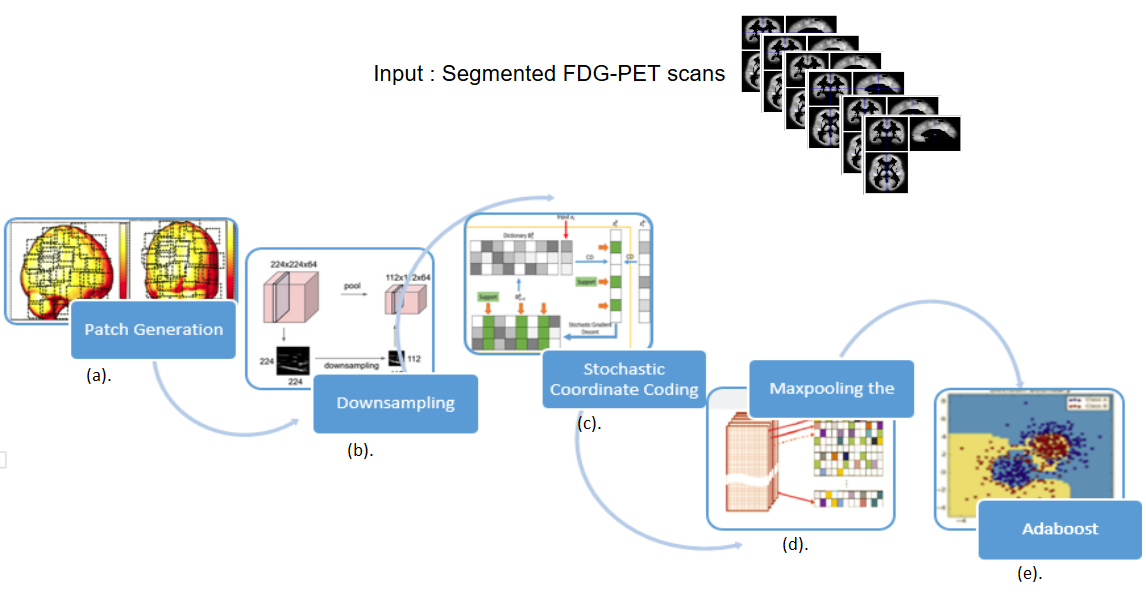
\includegraphics[width=\linewidth]{figures/pipeline1.png}
	\caption[Pipelines for Patch based Stochastic Coordinate Coding]{Pipelines for patch based Stochastic Coordinate Coding. (a). Patches are generated for feature extraction. (b). The size of patch dimension is reduced (c). After linearly arranging all the patches we find the dictionary and the sparse codes. (d). Maxpooling the learned sparse codes for obtaining a objective matrix. (e).applying AdaBoost for classification.}
	\label{fig:pipeline1}
\end{figure}

\begin{figure}[h]
	\centering
	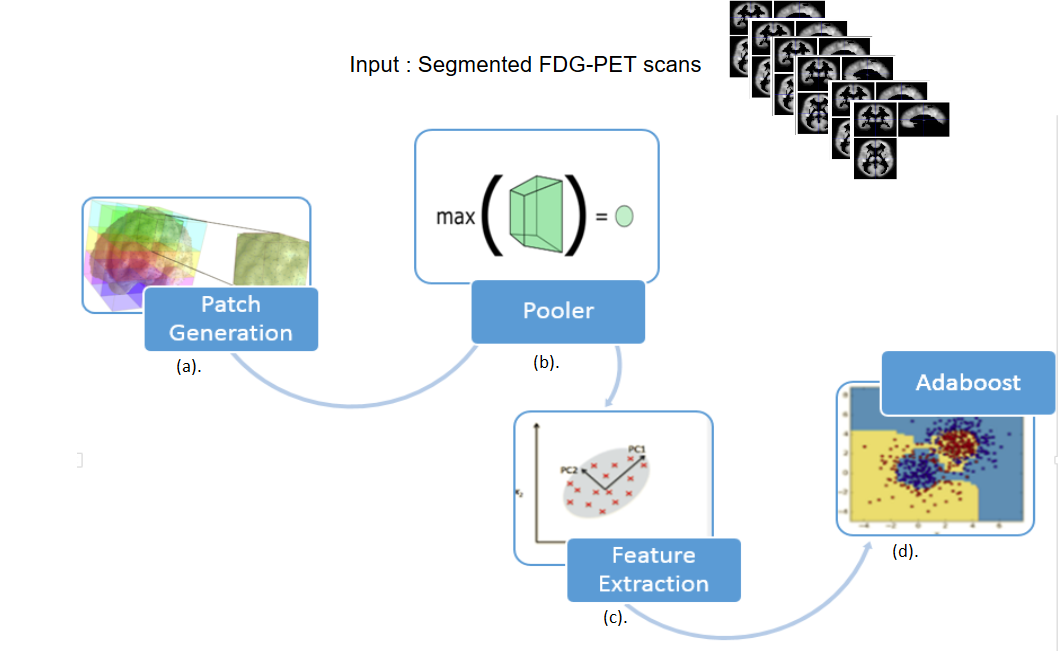
\includegraphics[width=\linewidth]{figures/pipeline2.png}
	\caption[Pipelines for Patch based Feature Extraction]{Pipelines for patch based feature extraction, (a). patches are generated for feature extraction. (b). patches are pooled to obtain specific activation. (c). the pooled values are linearly arranged and PCA is used to reduce it to a lower dimension space. (d). Adaboost is applied on the new feature space.}
	\label{fig:pipeline2}
\end{figure}

\section{Assumptions}
In both our methods we have made certain assumptions while building the system. This section describes the assumptions and to what extent they hold true 
\begin{enumerate}
\item \textit{The sample of the population is a representative sample.}\\
We assume the sample provided by the ADNI initiative is representative of the the population. The representative sample allows the collected results to be generalized to a larger population. We assume the \FDGPET~ analysis can be generalized to the general population.
\item \textit{3D Patch pooling represents the activation of a volume.}\\
In our first method of classification we use patch statistics to build the feature matrix with an assumption that the aggregate volume's (under $ 10\times10\times10 $) activation can be represented by the maximum intensity of the voxel within that region.   
\item \textit{The cerebral cortex intensities are assumed to serve as a biomarker.}\\
In this study we assume that the entire cerebral cortex may relay the metabolic information. In previous years z-score based t-values have been calculated to study regions of the brain and theory states that the metabolic changes during disease progression have a differential effect on various parts of the brain~\citep{ishii2014pet}. This is a benign analysis and we assume cerebral cortex is can serve as a good biomarker. 
\end{enumerate}

\chapter{Experiments and Results} %experimental results
We set up our system  on ``Saguaro'' one of the three computing environments provided by ASU for research purposes. Saguaro is a 5K processor Dell Linux cluster which can perform almost 45 million floating point operation per second, it has over 9 Tera bytes of RAM and over 400 Terra Bytes aggregate disk space. A node on Saguaro can be easily and conveniently accessed via a SSH protocol. Each node has 8 processors and 16GB of RAM. I acquired a node on saguaro during the summer of 2015.

\section{Experimental Setup}
In prior work ~\cite{zhang2016applying} the authors study the surface deformation of the hippocampal region of the brain and use it as features for training a dictionary of basis vectors and associated sparse codes. This encoding learn sets of over complete basis vectors which are better able to capture structures and patterns inherent in the input data. The hippocampal surface is modeled from the hippocampal region of the brain and patches on its surface captures topological information effectively. Similar a system can be designed which uses a patch based feature extraction process and then use statistics derives form the patches for classification. However an important question for diagnostic classification based on voxel-based or surface-based maps is which statistics are best to analyze. 

\citep{kakimoto2011new} used the total z-score from the Brodmann Area sensitivity map in the brain surface, ~\citep{lu2017early} calculated the mean voxel values from 116 VOIs, standard deviations of voxel values from the 116 anatomical VOIs, and mean voxel value differences between 54 pairs of the anatomical VOIs on left and right brain hemispheres. All VOIs were extracted form a AAL template similar to the one in Fig.~\ref{fig:mask} with more regions of varying intensities. We hypothesize that a patch based extraction methods which selects overlapping volumes from each image in a number of samples and learns there sparse representations via a dictionary can then be used for classification Alg.~\ref{alg:pipeline1}. To compare this system we design one more system Alg.~\ref{alg:pipeline2} in which we directly pool intensities in the patch volume to a max. Maxing the overlapping patches ensure that the activation around a region is local to that volume. After which PCA can be applied to reduce the high dimension of the data and also helps in reducing noise induced for the blank patches (covering no region). We then evaluate the cerebral cortex as a potential imaging biomarker for AD diagnosis and prognosis research.  

The two systems we come up with are described below : 
\begin{enumerate}
	\item  Patch based Stochastic Coordinate Coding, Pooling the sparse codes to generate features for annotation, boosting features by adding gender, age, \apoe{1}, \apoe{2} and FAQ followed by classification. 
	\item Pooling $ n $ patches, using gender, age, \apoe{1}, \apoe{2} and FAQ as additional features for boosting classification, reducing the dimensions of the annotated patches and classification. 
\end{enumerate}

After normalizing, segmenting and skull stripping the cerebral cortex we extract features for classification.  In our experiments each processed FDG-PET is a $ 80 \times 95 \times 80 $ image with intensity values spread over the voxel volume. In this study we applied two different patch based extraction techniques. (1) For patch based sparse coding we compared 500, 1000 and 2000 number of patches to make the objective matrix for SCC. To reduce complexity we down sample 1000 dimensional patches to 125 dimensions by using a $ 2 \times 2 \times 2 $ window as described in Sec.~\ref{subsec:Patch_Generation_Dictionary_Learning}. (2) For patch based dimension reduction (PPCA) we made $ 4050 $ patches with varying overlap across the cerebral ROI-segmented FDG-PET volume. Fig.~\ref{fig:patches}(a,b) shows the patch formation for (1) and (2).

\begin{figure}
	\centering
	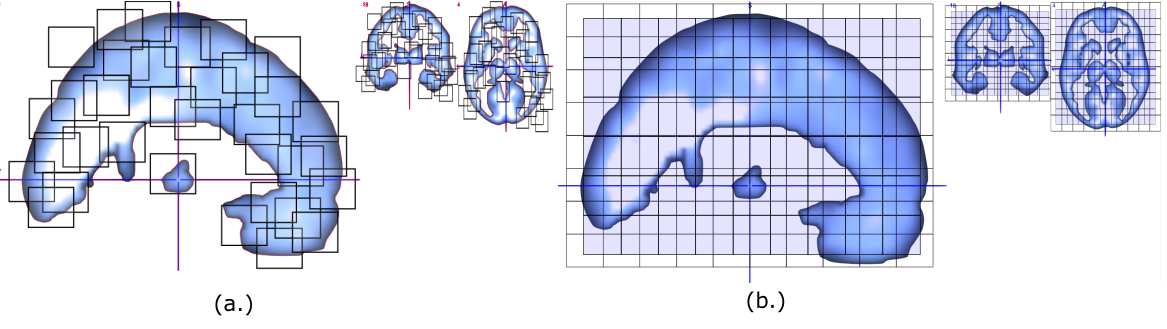
\includegraphics[width=\linewidth]{figures/patches}
	\caption[Unstructured and Structured patches in Axial, Sagittal and Coronal view of the brain.]{(a). Unstructured patches in Alg.1. The patches are generated randomly and ensure overlapping by creating enough of them. (b). Structured patches in Alg.2. with overlap shown in a slightly stronger shade of blue.}
	\label{fig:patches}
\end{figure}

In the training matrix we then involve additional features which enables us to make well defined classification, we include the genetic information and Functional Activities Questionnaire (FAQ) Scores even Age and Gender were involved. the two alleles of Apolipoprotein E(APOE) are available, APOE genotype is represented by combination of $e2$ (episilon 2),$e3$ and $e4$. Each individual will have one of the following combinations: $e2/e2$, $e2/e34$, $e2/e44$, $e3/e3$, $e3/e4$, $e4/e4$. Although the order between two genotypes for each person doesn't matter, they are represented in the order of $e2 \ge e3 \ge e4$. After feature annotation, the dimension of the dataset was reduced to a reasonable size and classification was performed.

\subsection{System Configuration}
We manage the data files on the cluster and use two system for the designing of both our systems. 

\begin{table}[h]
	\centering
	\begin{tabular}{|P{6cm}|P{7cm}|}
		\hline
		\multirow{4}*{Dell PowerEdge T110 II Server}
		& CPU : Intel Core2 Quad @ 2.6 GHz\\
		& OS : Windows 7\\
		&Total Memory (RAM) : 8 GB\\
		&No. of Cores : 4\\
		\midrule
		\multirow{4}*{Dell Alienware X1} 
		& CPU : Intel Core i5 @ 2.8 GHz\\
		& OS : Windows 10\\
		&Total Memory (RAM) : 16 GB\\ 
		&No. of Cores : 4\\
		\hline
	\end{tabular}
	\caption{system configurations}
	\label{tab:system configurations}
\end{table}

\subsection{Languages and Software used.}
In this section we enumerate the software tools and languages used for the experiments.
\begin{enumerate}
\item Matlab (2016a,2015b) : To make the patches in both experiment \textbullet~ To max-pool the data in patch pooling and down-sampling the patches in (SCC) Section.~\ref{subsec:Patch_Generation_Dictionary_Learning}.  
\item C++ : To pool the learned dictionary \textbullet~ Sparse Coding, the code os taken from ~\citep{lin2014stochastic} and modified to fit our needs.
\item Python~(2.7.12) : For classification and file management
\item Shell : for scripting the above listed.
\item Software : SPM To preprocess the \FDGPET~ scans \textbullet~ InkScape for diagrams \textbullet~ Micron: for visualizing NiFTI files \textbullet ~MobaXterm / WinSCP / Putty: For accessing the cluster
\item Libraries : Python/2.7.12 (sklearn) for classifiers.
\end{enumerate}


 \section{Results}
\label{sec:Results}
We run six experiments over the two methods described in Algorithm~\ref{alg:pipeline1} (1) and Algorithm~\ref{alg:pipeline2} (2). An N-fold cross validation protocol was adopted to estimate classification accuracy. All subjects were randomly divided into N folds. The surface biomarkers were selected by training on N-1 folds and the test was performed on the remaining fold. We rotated this procedure for N times to estimate the accuracy. In this paper, we choose N = 10 to complete the classification.The output of each classification experiment was compared to the ground truth, and a contingency table was computed to indicate how many class labels were correctly identified as members of one of the two classes. The rows of the contingency table represent the true classes and the columns represent the assigned classes. The cell at row r and column $c$ is the number of subjects whose true class is r while their assigned class is $c$. Natural performance measures for classification problems mainly based on error rate or accuracy. However, higher accuracy does not necessarily imply better performance on target task. In two-category classification, one method for handling $c$-class problem is to consider $c$ 2-class problems: $ \frac{\omega_i}{not ~\omega_i} $~\citep{fawcett2004roc}. Therefore, confusion matrix was proposed as a method to measure classifier performance. TP, FP, TN, FN represents number of true positives, number of false positives, number of true negatives and number of false negative, respectively. The matrix in Table.~\ref{tab:confusion_matrix} represents a possible combination of ground truth and predicted classification for two classes.

\begin{table}[]
	\centering
	\begin{tabular}{|P{3.5cm}|P{3.5cm}|P{3.5cm}|}
		\hline
		& \multicolumn{2}{|P{7cm}|}{\emph{\bf Assigned Class}}\\
		\hline
		\emph{\bf True Class}& Positive & Negative \\
		\hline
		Positive & TP & FP \\
		Negative & FN & TN \\	
		\hline
	\end{tabular}
	\caption{Classification results between different classifiers}
	\label{tab:confusion_matrix}
\end{table}

The total of TP, FP, FN, TN refers to the total number in the classification. Five performance measures \F~Score, Recall, Specificity, Positive predictive value and Negative predictive value were calculated as follows:

\begin{equation*}
\textrm{F}_1~\textrm{Score} = 2 \times \frac{\textrm{TP}}{\textrm{FN} + 2\times \textrm{TP} + \textrm{FP}}.
\end{equation*}

In a given population precision measures the amount of true cases classified correctly and recall the strength of that number. When you have both high precision and high recall it would mean that the population is well classified. \F~Score is the measure that is the harmonic mean of precision and recall. The reason for taking harmonic mean is because it is more appropriate when dealing rates and ratios.  

\begin{equation*}
\textrm{Recall} = \frac{\textrm{TP}}{\textrm{TP} + \textrm{FN}}.
\end{equation*}

Recall in this context is also referred as the true positive rate or sensitivity.  is a statistical measure of how well a binary classification test correctly identifies a condition and the probability of correctly labeling members of the target class.

\begin{equation*}
\textrm{Specificity} = \frac{\textrm{TN}}{\textrm{FP} + \textrm{TN}}.
\end{equation*}

The specificity is a statistical measure of how well a binary classification test correctly identifies the negative cases.

\begin{equation*}
\textrm{Positive predictive value} = \frac{\textrm{TP}}{\textrm{TP} + \textrm{FP}}.
\end{equation*}

Where positive predictive value (PPV) is also referred to as precision, which measures the probability of a positive prediction is correct.

\begin{equation*}
\textrm{Negative predictive value} = \frac{\textrm{TN}}{\textrm{TN} + \textrm{FN}}.
\end{equation*}

which measures the probability of a negative prediction is correct.

All these measures provide relevant information about the classification and no single measure tells the entire story. For example consider a scenario where 90\% of the population does not have a disease and the 10\% population is misclassified by the classifier, the accuracy would still be 90\%. Thus we should use multiple measures.   

There are some standard performance evaluation measures for classification study. Bigger values usually mean stronger classification power. We also computed the area-under-the-curve (AUC) of the receiver operating characteristic (ROC). The ROC is the average value of sensitivity for all the possible values of specificity. Such an index is especially useful in a comparative study of two diagnostic tests. If two tests are to be compared, it is desirable to compare the entire ROC curve rather than at a particular point~\citep{swets1979roc}. The maximum AUC=1 means that the diagnostic test is perfect in the differentiation between the diseased and stable. This happens when the distribution of test results for the diseased and stable do not overlap. AUC = 0.5 means the chance of discrimination that curve located on diagonal line in ROC space. Using these measures of analysis we first report the comparison between different sets of feature, followed by a thorough analysis on both the proposed pipelines. We then list the AUC comparison in the end.

\subsection{Comparison between sets of features.}
We tested our best scores across the features we have have in store for classification. In this comparison we put emphasis on the features we are including in classification. We tested both the pipelines using (1).Voxel information from the image (2). Voxels combined with rich genetic scores described in section.\ref{sec:Results} (3). A combination of (2) and the other demographic information. We observe that (3). gives very good results in AD vs. CU $ \sim 98\% $. Only in CU vs. LMCI (2) performs better with $ \sim 82 \% $    
\begin{table}[!h]
	\centering
	\begin{tabular}{P{3cm}P{3cm}P{2cm}P{3cm}P{3cm}}
		\hline
		Methods&Exp.& Voxels & Voxels + \apoe{2} + \apoe{3} + FAQ &  Voxels + \apoe{2} + \apoe{3} + FAQ + Age~\& Gender\\\hline
		\multirow{6}{*}{Pool+FE}
		& AD vs. CU		&$ 88.97 $&$ 95.10  $&$ 96.30 $\\
		& AD vs. EMCI 	&$ 76.92 $&$ 81.69 $&$ 83.68 $\\
		& AD vs. LMCI	&$ 63.26 $&$ 69.44 $&$ 73.42 $\\
		& CU vs. EMCI	&$ 54.49 $&$ 62.63 $&$ 69.94 $\\
		& CU vs. LMCI	&$ 63.87 $&$ 82.19 $&$ 78.28 $\\
		& EMCI vs. LMCI	&$ 58.04 $&$ 59.47 $&$ 57.38 $\\
		\midrule
		\multirow{6}{*}{SCC}
		& AD vs. CU		&$ 81.69 $&$ 95.78 $&$ 95.78 $\\
		& AD vs. EMCI 	&$ 74.56 $&$ 81.31 $&$ 81.31 $\\
		& AD vs. LMCI	&$ 64.44 $&$ 78.49 $&$ 78.49 $\\
		& CU vs. EMCI	&$ 51.96 $&$ 59.57 $&$ 64.02 $\\
		& CU vs. LMCI	&$ 61.37 $&$ 63.89 $&$ 79.58 $\\
		& EMCI vs. LMCI	&$ 51.96 $&$ 59.05 $&$ 59.05 $\\
		\hline
	\end{tabular}
	\caption{Classification results between different feat F1-measures}
	\label{tab:comparision_features}
\end{table}

\subsection{Pooling and Dimension Reduction}
\label{subsec:extraction}
We tested the framework described in Alg.~\ref{alg:pipeline1} in six classification experiments (1). AD vs CU, (2). AD vs EMCI, (3). AD vs LMCI, (4). CU vs EMCI, (5). CU vs LMCI and (6). CU vs EMCI. We made $ 4050 $ patches and we extracted the Age, Gender, Apo$E$2\footnote{https://www.ncbi.nlm.nih.gov/pmc/articles/PMC1243648/}~\citep{ghebranious2005detection,genin2011apoe}, Apo$E$3, and Functional Activities Questionnaire (FAQ) Scores for each sample for the purpose of comparison. To boost classification we use the combination of ``Voxel Feature'', ``Apo$E$2'', ``Apoe$E$3'', ``FAQ'', ``Age'' and ``Gender''. We test the accuracy of using only the voxels as features against using (voxels + Apo$ E $2 + Apoe$E$3 + FAQ) and (voxels + Apoe$E$2 + Apoe$ E $3 + FAQ + Age and Gender). The classification results are shown in Table.~\ref{tab:comparision_features}.
As seen in  Table.~\ref{tab:comparision_features} using the combination of all the features (Voxels, Apo$E$2, Apo$E$3, FAQ, Age, Gender) gave the best results.
To correctly classify the annotated features we use dimension reduction before classification to avoid overfitting. We compare Principle Component Analysis (PCA), Singular Value Decomposition (SVD) and Kernel PCA (KPCA).~\citep{mika1998kernel}. 
For the purpose of classification we choose AdaBoost~\citep*{shawe2004kernel} and compare it with popularly used classifiers such as Nears Neighbor, Linear Singular Valued Decomposition (Linear SVD), Gaussian Process (GP)~\citep{rasmussen2006gaussian} and AdaBoost~\citep{rojas2009adaboost}. 

\textit{Comparison between different classifiers}\\
As indicated in Table.~\ref{tab:comparision_classifiers} the \F~Score of AD vs CU is best for Gaussian Process (GP) with a $ 97.3 \% $ \F~Score compared to $ 96.2 \% $ in AdaBoost. $ 98.38 \% $ PPV and $ 95.20 \% $ NPV indicates both the classes have been effectively classified. The class separation is maximum in case of AD vs CU in reference to disease progression that explains the high \F measure. For AD vs EMCI, AD vs LMCI, CU vs EMCI and CU vs LMCI the \F Score is highest case of Gaussian Process. In case of CU vs LMCI AdaBoost performs comparatively poor in comparison to other classifiers. For EMCI vs LMCI the NPV is poor for GP and Linear SVM which means one class is poorly classifier and the classification accuracy is inconsistent. In this case AdaBoost performed good as it gave a more consistent NPV and PPV the recall and sensitivity is also the best in this experiment. For further comparison between dimensionality reduction we keep our classifier as AdaBoost because of a more correct classification when AdaBoost was used as classifier across all the experiments.   

\begin{table}[!h]
	\centering
	\begin{tabular}{P{3cm}P{2.5cm}P{1.25cm}P{1.25cm}P{1.25cm}P{1.25cm}P{1.25cm}P{1.25cm}}
		\hline
		Measure&Method& AD \ CU & AD \ EMCI & AD \ LMCI & CU \ EMCI & CU \ LMCI & LMCI \ EMCI \\\hline
		\multirow{4}{*}{Nearest Neighbor}
		& F1 Score		&$ 96.53 $&$ 83.33 $&$ 75.98 $&$ 73.65 $&$ 84.87 $&$ 60.77 $\\
		& Recall		&$ 95.76 $&$ 88.46 $&$ 79.69 $&$ 67.41 $&$ 77.67 $&$ 56.52 $\\
		& Specificity	&$ 96.50 $&$ 84.02 $&$ 76.60 $&$ 75.00 $&$ 90.00 $&$ 52.71 $\\
		& PPV			&$ 97.31 $&$ 78.76 $&$ 72.60 $&$ 81.18 $&$ 93.54 $&$ 65.73 $\\
		& NPV			&$ 94.52 $&$ 91.57 $&$ 82.91 $&$ 58.98 $&$ 68.35 $&$ 43.03 $\\
		\midrule
		\multirow{4}{*}{Linear SVM}
		& F1 Score		&$ 96.79 $&$ 83.27 $&$ 77.35 $&$ 75.79 $&$ 84.95 $&$ 67.27 $\\		
		& Recall		&$ 96.27 $&$ 86.67 $&$ 78.72 $&$ 65.87 $&$ 77.43 $&$ 56.75 $\\
		& Specificity	&$ 96.52 $&$ 84.65 $&$ 78.52 $&$ 82.14 $&$ 90.67 $&$ 59.74 $\\
		& PPV			&$ 97.31 $&$ 80.13 $&$ 76.02 $&$ 89.24 $&$ 94.08 $&$ 82.58 $\\
		& NPV			&$ 95.20 $&$ 89.88 $&$ 81.01 $&$ 51.68 $&$ 67.72 $&$ 29.11 $\\
		\midrule
		\multirow{4}{*}{Gaussian Process}
		& F1 Score		&$ 97.34 $&$ 83.68 $&$ 77.58 $&$ 75.96 $&$ 85.64 $&$ 63.76 $\\
		& Recall		&$ 96.31 $&$ 86.76 $&$ 80.74 $&$ 68.69 $&$ 79.35 $&$ 55.93 $\\
		& Specificity	&$ 97.88 $&$ 85.10 $&$ 78.10 $&$ 79.10 $&$ 89.68 $&$ 54.00 $\\
		& PPV			&$ 98.38 $&$ 80.82 $&$ 74.65 $&$ 84.94 $&$ 93.01 $&$ 74.15 $\\		
		& NPV			&$ 95.20 $&$ 89.88 $&$ 83.54 $&$ 59.55 $&$ 71.51 $&$ 34.17 $\\		
		\midrule
		\multirow{4}{*}{AdaBoost}
		& F1 Score		&$ 96.85 $&$ 83.33 $&$ 73.42 $&$ 69.94 $&$ 78.28 $&$ 57.38 $\\
		& Recall		&$ 94.38 $&$ 84.50 $&$ 75.00 $&$ 67.50 $&$ 78.07 $&$ 58.04 $\\
		& Specificity	&$ 99.26 $&$ 85.71 $&$ 75.00 $&$ 58.90 $&$ 74.52 $&$ 52.46 $\\
		& PPV			&$ 99.46 $&$ 82.19 $&$ 71.91 $&$ 72.58 $&$ 78.49 $&$ 56.74 $\\
		& NPV			&$ 92.46 $&$ 87.64 $&$ 77.85 $&$ 63.48 $&$ 74.40 $&$ 53.79 $\\				
		\hline
	\end{tabular}
	\caption{Classification results between different classifiers}
	\label{tab:comparision_classifiers}
\end{table}

\textit{Comparing different Dimension reduction techniques,}\\
As indicated in Table.~\ref{tab:comparision_dimension_reduction} the \F~Score of AD vs CU is best when the dimensions are reduced using singular valued decomposition (SVD) with \acc{97} \F~Score. The high Recall and Specificity implies AD vs CU is well classified. Again we believe the \FDGPET~biomarker along with \apoe{2} and \apoe{3} the two alleles of Apolipoprotein E and the Functional Activities Questionnaire (FAQ) are extremely sensitivity if classifying between \Alzheimers and Normal Control. 
Column two in \Tbl{tab:comparision_dimension_reduction} shows that the subjects in AD vs EMCI are separable to a good extent with \F~Score of \acc{83.3} in case of Principle Component Analysis (PCA) and a Recall of \acc{84.5} and Specificity of \acc{85.7} shows that both the classes have been evenly separated. 
Kernel PCA~\citep{mika1998kernel} performed the best in remaining experiments. With CU vs LMCI the group separation is of one i.e. the disease progression there is one stage in between CU and LMCI and we observe in column 5 of Table.~\ref{tab:comparision_dimension_reduction} the \F~Score is \acc{80}. With AD vs LMCI and CU s EMCI with Kernel PCA the \F~Score is \acc{76.65} and \acc{71.46} respectively. The last experiment (LMCI vs EMCI) \F~Score of \acc{60.3} is the most difficult to classify many good and popular classifiers failed to classify the complex nature of early Mild impairment (EMCI) and impairment (LMCI). EMCI and LMCI as described in Section~\ref{subjects} are derived from the Mild Cognitive Impairment (MCI) stage in ADNI1 and the participants reported a subjective memory concern the difference in EMCI and LMCI is decided by the Wechsler Memory Scale Logical (WMS). We believe there is no clear separation with \FDGPET~ as our biomarker and maybe more specific ROI may lead us to a more concrete conclusion. 

\begin{table}[!h]
	\centering
	\begin{tabular}{P{2.25cm}P{2.5cm}P{1.25cm}P{1.25cm}P{1.25cm}P{1.25cm}P{1.25cm}P{1.25cm}}
		\hline
		Measure&Method& AD \ CU & AD \ EMCI & AD \ LMCI & CU \ EMCI & CU \ LMCI & LMCI \ EMCI \\\hline
		\multirow{5}{*}{PCA}
		& F1 Score		&$ 96.85 $&$ 83.33 $&$ 73.42 $&$ 69.94 $&$ 78.28 $&$ 57.38 $\\
		& Recall		&$ 94.38 $&$ 84.50 $&$ 75.00 $&$ 67.50 $&$ 78.07 $&$ 58.04 $\\
		& Specificity	&$ 99.26 $&$ 85.71 $&$ 75.00 $&$ 58.90 $&$ 74.52 $&$ 52.46 $\\
		& PPV			&$ 99.46 $&$ 82.19 $&$ 71.91 $&$ 72.58 $&$ 78.49 $&$ 56.74 $\\
		& NPV			&$ 92.46 $&$ 87.64 $&$ 77.85 $&$ 63.48 $&$ 74.40 $&$ 53.79 $\\
		\midrule
		\multirow{5}{*}{SVD}
		& F1 Score		&$ 97.09 $&$ 81.85 $&$ 70.23 $&$ 66.67 $&$ 77.62 $&$ 57.47 $\\
		& Recall		&$ 95.33 $&$ 85.18 $&$ 68.62 $&$ 67.78 $&$ 77.83 $&$ 58.82 $\\
		& Specificity	&$ 98.56 $&$ 83.59 $&$ 72.19 $&$ 65.59 $&$ 73.58 $&$ 53.01 $\\
		& PPV			&$ 98.92 $&$ 78.76 $&$ 71.91 $&$ 65.59 $&$ 77.41 $&$ 56.17 $\\
		& NPV			&$ 93.83 $&$ 88.76 $&$ 69.62 $&$ 67.41 $&$ 74.05 $&$ 55.69 $\\	
		\midrule
		\multirow{5}{*}{Kernel PCA}
		& F1 Score		&$ 96.65 $&$ 82.47 $&$ 76.65 $&$ 71.46 $&$ 80.01 $&$ 60.39 $\\
		& Recall		&$ 95.77 $&$ 82.75 $&$ 78.01 $&$ 68.47 $&$ 78.06 $&$ 59.56 $\\
		& Specificity	&$ 96.50 $&$ 85.47 $&$ 77.91 $&$ 70.80 $&$ 77.02 $&$ 54.90 $\\
		& PPV			&$ 97.31 $&$ 82.19 $&$ 75.34 $&$ 74.73 $&$ 82.25 $&$ 61.23 $\\
		& NPV			&$ 94.52 $&$ 85.95 $&$ 80.37 $&$ 64.04 $&$ 72.78 $&$ 53.16 $\\
		\hline
	\end{tabular}
	\caption{classification results with PCA, SVD and Kernel PCA (classifier : AD)}
	\label{tab:comparision_dimension_reduction}
\end{table}


\subsection{Patch based  Stochastic Coordinate Coding}
\label{subsec:patch_based_scc}
Having learned and classified the features using traditional feature extraction techniques we use another dimensionality reduction approach, Stochastic Coordinate Coding described in Section~\ref{subsec:theoritical_background} to learn a dictionary which allows us to store images more efficiently as a superposition of a small number of its elements so that each image is reduced to a small number of coefficient. 
We tested the framework described in Alg.~\ref{alg:pipeline2} in six classification experiments (1). AD vs CU, (2). AD vs EMCI, (3). AD vs LMCI, (4). CU vs EMCI, (5). CU vs LMCI and (6). CU vs EMCI. We made $ 8000 $ patches across the entire \FDGPET~Cerebral cortex to ensure overlapping and then selected $ 1000 $ random patches for initializing the dictionary. The sample size for AD vs CU, AD vs EMCI, AD vs LMCI, CU vs EMCI, CU vs LMCI and  vs EMCI is $ 332000 $, $ 324000 $, $ 304000 $, $ 344000 $,  $ 364000 $ and $ 336000 $. Our choice of patch size is $ 10\times 10\times 10 $ and the sample $ \times $ feature size for say AD vs CU is $ 344,000,000 $ which is a huge problem size, to tone down our features we down-sample the $ 10\times 10\times 10 $ patches by a $ 2\times 2\times 2 $ kernel and reduce the samples to $ 125 $. Figure.~\ref{fig:maxpooling}(b) shows the general idea of downsampling. After learning the 2000 dimension dictionary and sparse codes were learned, we applied max-pooling~\citep{scherer2010evaluation} to generate features for annotation. After feature reduction, the dimension of the dataset was reduced to a reasonable size and classification was performed.

Yet again we extract the Age, Gender, Apo$E$2\footnote{https://www.ncbi.nlm.nih.gov/pmc/articles/PMC1243648/}~\citep{ghebranious2005detection,genin2011apoe}, Apo$E$3, and Functional Activities Questionnaire (FAQ) Scores for each sample for the purpose of comparison. To boost classification we use the combination of ``Voxel Feature'', ``Apo$E$2'', ``Apoe$E$3'', ``FAQ'', ``Age'' and ``Gender''. We test the accuracy of using only the voxels as features against using (voxels + Apo$ E $2 + Apoe$E$3 + FAQ) and (voxels + Apoe$E$2 + Apoe$ E $3 + FAQ + Age and Gender). The classification results are shown in Table.~\ref{tab:comparision_features}.
As seen in  Table.~\ref{tab:comparision_features} using the combination of all the features (Voxels, Apo$E$2, Apo$E$3, FAQ, Age, Gender) gave the best results.
For the purpose of classification we choose AdaBoost~\citep*{shawe2004kernel} and compare it with popularly used classifiers such as Nears Neighbor, Linear Singular Valued Decomposition (Linear SVD), Gaussian Process (GP)~\citep{rasmussen2006gaussian} and AdaBoost~\citep{rojas2009adaboost}. 
We also vary the number of patches in the classification experiments we use $ 500,~1000,~1500,~2000$ patches. 


\textit{Comparison between different classifiers}\\
As indicated in Table.~\ref{tab:comparision_classifiers_scc} the \F~Score of AD vs CU is best for Gaussian Process (GP) with a \acc{97} \F~Score compared to \acc{96.7} in AdaBoost. \acc{98.3} PPV and \acc{94.2} NPV indicates both the classes have been effectively classified. The class separation is maximum in case of AD vs CU in reference to disease progression that explains the high \F measure. 
In case of experiments with a class separation of one i.e. AD vs EMCI and CU vs LMCI (column 2 and 5) Gaussian Process gives us the best results with \F~Score of \acc{83.27} and \acc{79.58}. In experiments with no class separability we see that AdaBoost and LinearSVM perform well with an \F~Score of \acc{78.5} in AD vs LMCI with AdaBoost and \F~Score of \acc{65.57} in CU vs EMCI with Linear SVM. 
As seen from Table.~\ref{tab:comparision_classifiers_scc} Gaussian Process gives a bad Recall Score for CU vs EMCI, CU vs LMCI and EMCI vs LMCI and we can see the NPV to be low indicating that the classifier fails to classify the experiments. In the latter cases Adaboost and Linear SVM performs evenly well for both classes and outperforms some unstable classifiers.     

\begin{table}[!h]
	\centering
	\begin{tabular}{P{3cm}p{2.5cm}p{1.25cm}p{1.25cm}p{1.25cm}p{1.25cm}p{1.25cm}p{1.25cm}}
		\hline
		Measure&Method& AD \ CU & AD \ EMCI & AD \ LMCI & CU \ EMCI & CU \ LMCI & LMCI \ EMCI \\\hline
		\multirow{4}{*}{Nearest Neighbor}
		& F1 Score		&$ 97.05 $&$ 79.02 $&$ 74.91 $&$ 73.23 $&$ 83.80 $&$ 59.73 $\\
		& Recall		&$ 96.79 $&$ 80.71 $&$ 77.37 $&$ 65.00 $&$ 75.21 $&$ 56.85 $\\
		& Specificity	&$ 96.55 $&$ 82.06 $&$ 76.04 $&$ 75.80 $&$ 90.91 $&$ 52.51 $\\
		& PPV			&$ 97.31 $&$ 77.39 $&$ 72.60 $&$ 83.38 $&$ 94.62 $&$ 62.92 $\\
		& NPV			&$ 95.89 $&$ 84.83 $&$ 80.04 $&$ 52.80 $&$ 63.29 $&$ 46.20 $\\
		\midrule
		\multirow{4}{*}{Linear SVM}
		& F1 Score		&$ 96.80 $&$ 81.78 $&$ 74.56 $&$ 65.04 $&$ 81.74 $&$ 60.38 $\\		
		& Recall		&$ 95.78 $&$ 82.06 $&$ 75.88 $&$ 65.57 $&$ 78.32 $&$ 59.56 $\\
		& Specificity	&$ 97.18 $&$ 84.91 $&$ 76.07 $&$ 63.53 $&$ 80.48 $&$ 54.90 $\\
		& PPV			&$ 97.84 $&$ 81.50 $&$ 73.28 $&$ 64.51 $&$ 85.48 $&$ 62.23 $\\
		& NPV			&$ 94.52 $&$ 85.39 $&$ 78.48 $&$ 64.60 $&$ 72.15 $&$ 53.16 $\\
		\midrule
		\multirow{4}{*}{Gaussian Process}
		& F1 Score		&$ 97.08 $&$ 83.27 $&$ 76.70 $&$ 73.44 $&$ 73.30 $&$ 64.05 $\\
		& Recall		&$ 95.81 $&$ 86.27 $&$ 80.45 $&$ 59.79 $&$ 58.22 $&$ 56.70 $\\
		& Specificity	&$ 97.87 $&$ 84.65 $&$ 77.19 $&$ 86.76 $&$ 92.85 $&$ 55.23 $\\
		& PPV			&$ 98.38 $&$ 80.13 $&$ 73.28 $&$ 95.16 $&$ 98.92 $&$ 73.59 $\\		
		& NPV			&$ 94.20 $&$ 89.88 $&$ 83.54 $&$ 33.14 $&$ 16.41 $&$ 36.70 $\\		
		\midrule
		\multirow{4}{*}{AdaBoost}
		& F1 Score		&$ 95.78 $&$ 81.31 $&$ 78.49 $&$ 64.02 $&$ 79.58 $&$ 59.05 $\\
		& Recall		&$ 93.81 $&$ 87.40 $&$ 78.23 $&$ 63.02 $&$ 76.66 $&$ 58.56 $\\
		& Specificity	&$ 97.10 $&$ 82.23 $&$ 80.02 $&$ 62.05 $&$ 77.62 $&$ 53.54 $\\
		& PPV			&$ 97.84 $&$ 76.02 $&$ 78.76 $&$ 65.05 $&$ 82.79 $&$ 59.55 $\\
		& NPV			&$ 91.78 $&$ 91.01 $&$ 79.74 $&$ 60.11 $&$ 70.25 $&$ 52.53 $\\	
		\hline
	\end{tabular}
	\caption{Classification results between different classifiers}
	\label{tab:comparision_classifiers_scc}
\end{table}

\textit{Comparing different number of features}\\
In this comparison we refrain the results of experiments to only the voxel feature. We are more interested in the performance of SCC when the number of random patches are varied with regards to simplifying the image. The other factors responsible for boosting classification  essentially acts as non-factors if we wish to study dictionary learning for feature learning. As indicated in Table.~\ref{tab:comparision_features_scc} the \F~Score of AD vs CU is best when the number of features are more.

\begin{table}[!h]
	\centering
	\begin{tabular}{P{2.25cm}P{2.5cm}P{1.25cm}P{1.25cm}P{1.25cm}P{1.25cm}P{1.25cm}P{1.25cm}}
		\hline
		Measure&Method& AD \ CU & AD \ EMCI & AD \ LMCI & CU \ EMCI & CU \ LMCI & LMCI \ EMCI \\\hline
		\multirow{5}{*}{500 F}
		& F1 Score		&$ 96.82 $&$ 82.51 $&$ 71.94 $&$ 64.70 $&$ 78.30 $&$ 61.53 $\\
		& Recall		&$ 95.31 $&$ 84.28 $&$ 75.75 $&$ 64.36 $&$ 77.08 $&$ 60.21 $\\
		& Specificity	&$ 97.86 $&$ 84.78 $&$ 73.25 $&$ 63.06 $&$ 75.00 $&$ 56.00 $\\
		& PPV			&$ 98.38 $&$ 80.82 $&$ 68.49 $&$ 65.03 $&$ 79.56 $&$ 62.90 $\\
		& NPV			&$ 93.83 $&$ 87.64 $&$ 79.74 $&$ 62.35 $&$ 72.15 $&$ 53.16 $\\
		\midrule
		\multirow{5}{*}{1000 F}
		& F1 Score		&$ 96.29 $&$ 81.81 $&$ 77.39 $&$ 64.53 $&$ 74.40 $&$ 56.23 $\\
		& Recall		&$ 94.79 $&$ 83.57 $&$ 77.39 $&$ 64.02 $&$ 73.05 $&$ 53.26 $\\
		& Specificity	&$ 97.14 $&$ 84.57 $&$ 79.11 $&$ 62.85 $&$ 70.19 $&$ 47.44 $\\
		& PPV			&$ 97.84 $&$ 80.13 $&$ 77.39 $&$ 65.05 $&$ 75.80 $&$ 59.55 $\\
		& NPV			&$ 93.15 $&$ 87.07 $&$ 79.11 $&$ 61.79 $&$ 67.08 $&$ 41.13 $\\
		\midrule		   
		\multirow{5}{*}{2000 F}
		& F1 Score		&$ 97.35 $&$ 85.51 $&$ 75.60 $&$ 64.37 $&$ 77.17 $&$ 58.06$\\
		& Recall		&$ 95.83 $&$ 88.32 $&$ 75.86 $&$ 63.21 $&$ 78.02 $&$ 55.67 $\\
		& Specificity	&$ 98.57 $&$ 86.63 $&$ 77.35 $&$ 62.57 $&$ 72.83 $&$ 50.70 $\\
		& PPV			&$ 98.92 $&$ 82.87 $&$ 75.34 $&$ 65.59 $&$ 76.34 $&$ 60.67 $\\
		& NPV			&$ 94.52 $&$ 91.01 $&$ 77.84 $&$ 60.11 $&$ 74.68 $&$ 45.55 $\\
		\hline
		\end{tabular}
	\caption{classification results between number of patches in training the dictionary and sparse codes.}
	\label{tab:comparision_features_scc}
\end{table}

\subsection{AUC of ROC curves}
Area under the Curve is used to measure receiver operating characteristic (ROC) curve. The area is a measure of the predictive power of the classification experiment to classify a  randomly chosen positive example more accurately than a randomly chosen negative example. ROC is the graphical plot between the true positive rate and the false positive rate, it was first used during World War 2 for detecting enemy objects from friendly ships and noise. Know as Signal detection theory, it measures the ability of radar receiver operators to identify enemy ships. 

In this comparison we plot the AUC and compare both of our methods with and without demographics. The graphs show the superior accuracy of including rich features over only the regional voxel intensities. 
\begin{figure}
	\centering
	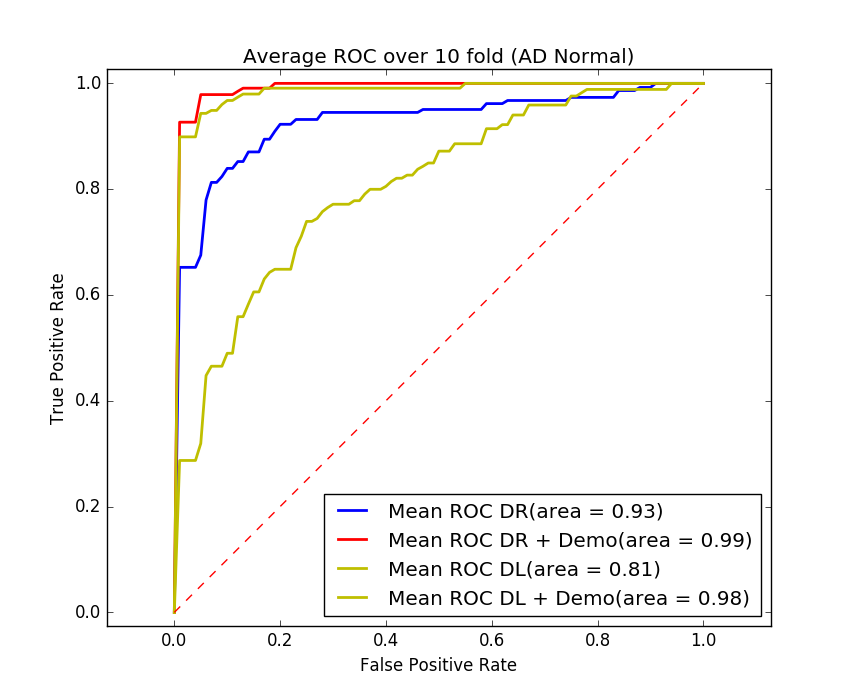
\includegraphics[width=\linewidth]{figures/AD_CU}
	\caption[ROC for AD vs. CU]{Classification in AD vs. CU group with different features performance comparison with receiver operating characteristic (ROC) curves and area under curve (AUC) measures. The results for RD, mTBM and MMS features are computed with the proposed PASS method. Within the three statistics, the result of using the MMS feature performs better than others. Among all AUC measures, MMS feature achieved the best performance (AUC = 0.78).}
	\label{fig:adcu}
\end{figure}
\begin{figure}
	\centering
	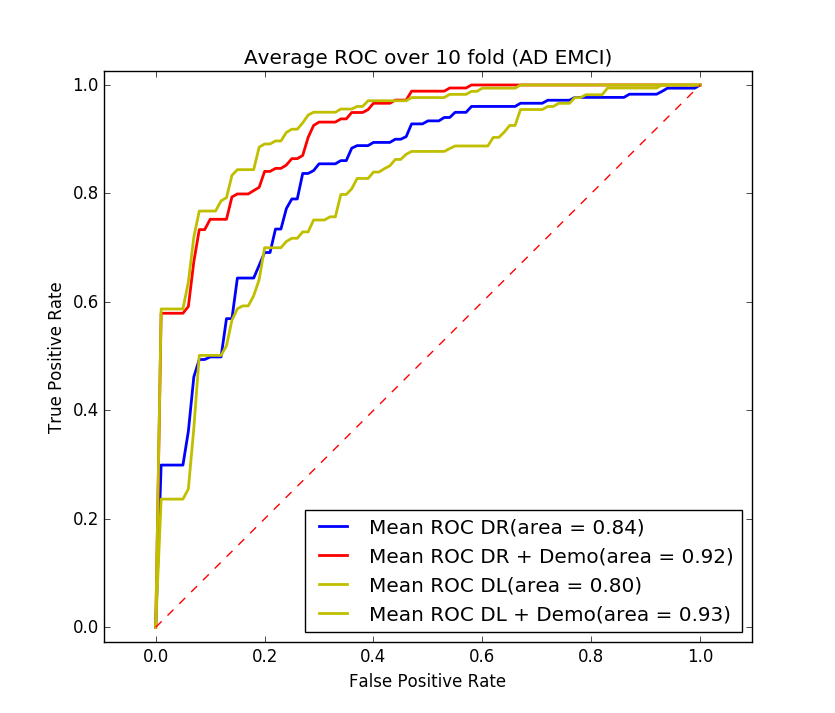
\includegraphics[width=\linewidth]{figures/AD_EMCI}
	\caption[ROC for AD vs. EMCI]{Classification in AD vs. CU group with different features performance comparison with receiver operating characteristic (ROC) curves and area under curve (AUC) measures. The results for RD, mTBM and MMS features are computed with the proposed PASS method. Within the three statistics, the result of using the MMS feature performs better than others. Among all AUC measures, MMS feature achieved the best performance (AUC = 0.78).}
	\label{fig:ademci}
\end{figure}
\begin{figure}
	\centering
	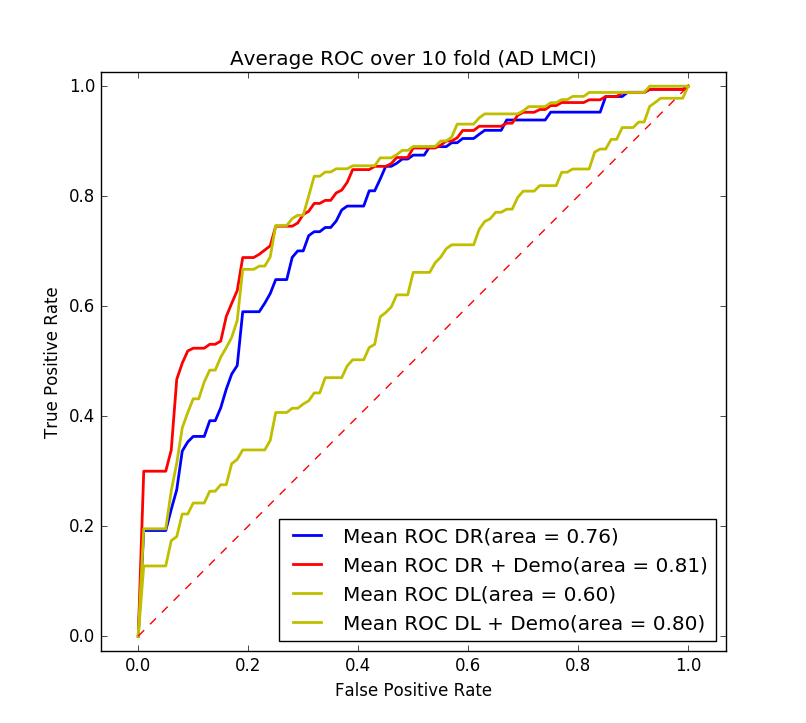
\includegraphics[width=\linewidth]{figures/AD_LMCI}
	\caption[ROC for AD vs. LMCI]{Classification in AD vs. CU group with different features performance comparison with receiver operating characteristic (ROC) curves and area under curve (AUC) measures. The results for RD, mTBM and MMS features are computed with the proposed PASS method. Within the three statistics, the result of using the MMS feature performs better than others. Among all AUC measures, MMS feature achieved the best performance (AUC = 0.78).}
	\label{fig:adlmci}
\end{figure}
\begin{figure}
	\centering
	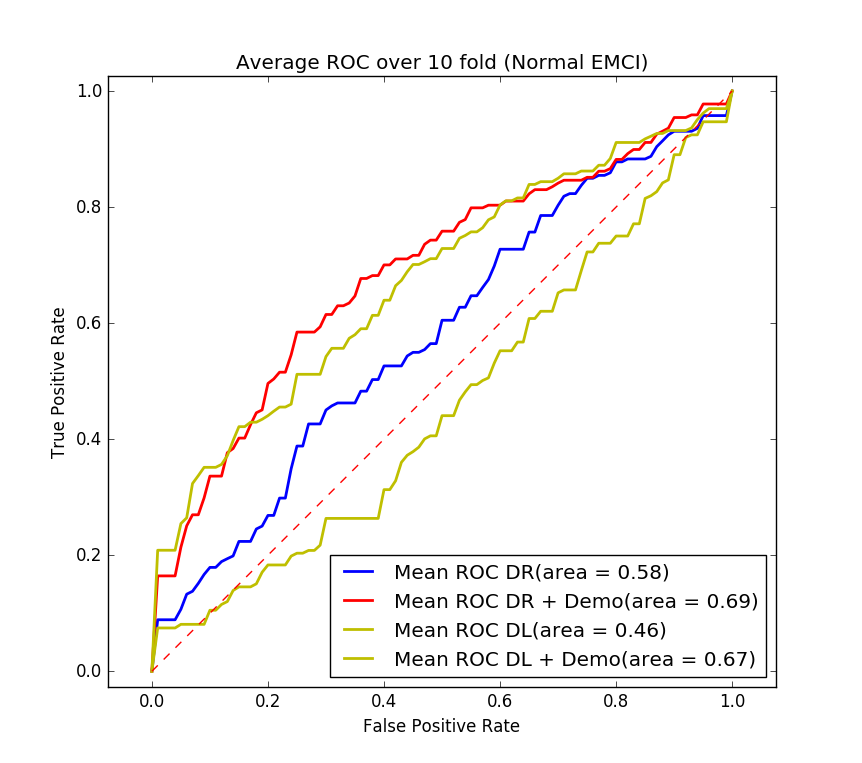
\includegraphics[width=\linewidth]{figures/CU_EMCI}
	\caption[ROC for Normal vs. EMCI]{Classification in AD vs. CU group with different features performance comparison with receiver operating characteristic (ROC) curves and area under curve (AUC) measures. The results for RD, mTBM and MMS features are computed with the proposed PASS method. Within the three statistics, the result of using the MMS feature performs better than others. Among all AUC measures, MMS feature achieved the best performance (AUC = 0.78).}
	\label{fig:cuemci}
\end{figure}
\begin{figure}
	\centering
	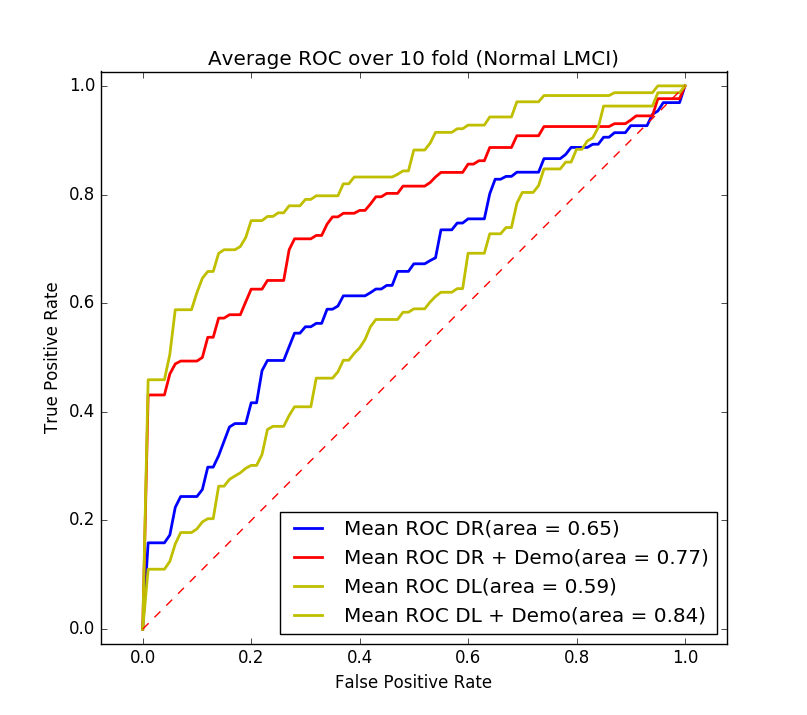
\includegraphics[width=\linewidth]{figures/CU_LMCI}
	\caption[ROC for Normal vs. LMCI]{Classification in AD vs. CU group with different features performance comparison with receiver operating characteristic (ROC) curves and area under curve (AUC) measures. The results for RD, mTBM and MMS features are computed with the proposed PASS method. Within the three statistics, the result of using the MMS feature performs better than others. Among all AUC measures, MMS feature achieved the best performance (AUC = 0.78).}
	\label{fig:culmci}
\end{figure}
\begin{figure}
	\centering
	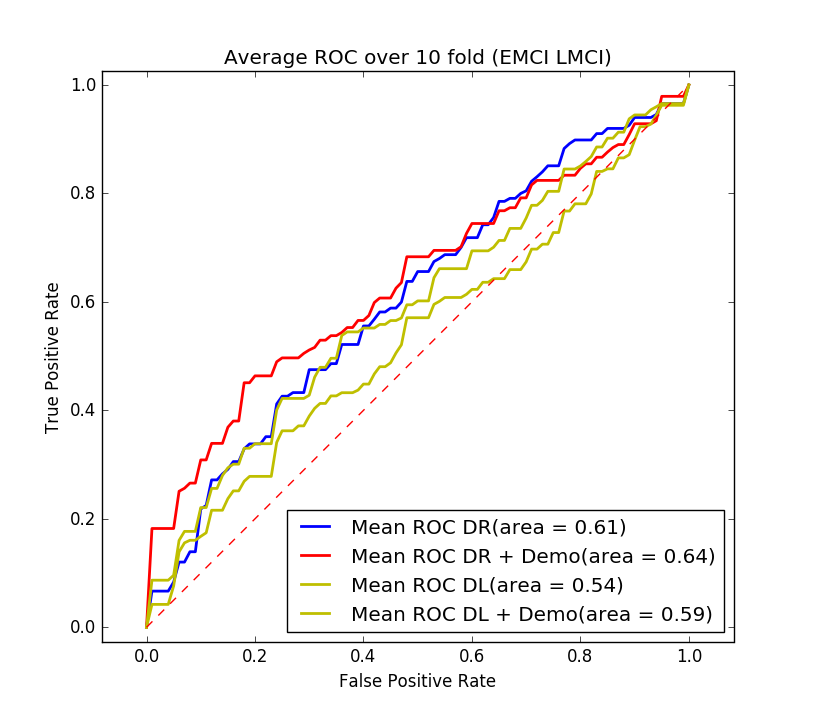
\includegraphics[width=\linewidth]{figures/EMCI_LMCI}
	\caption[ROC for EMCI vs. LMCI.]{Classification in AD vs. CU group with different features performance comparison with receiver operating characteristic (ROC) curves and area under curve (AUC) measures. The results for RD, mTBM and MMS features are computed with the proposed PASS method. Within the three statistics, the result of using the MMS feature performs better than others. Among all AUC measures, MMS feature achieved the best performance (AUC = 0.78).}
	\label{fig:emcilmci}
\end{figure}

\chapter{Discussion and Limitations}
Both the frameworks are are patch based differing in the extraction stage. The use of stochastic coordinate coding has been shown to work great with 3D surface data like MRI images ~\citep{zhang2016applying}. to model this system in voxel based 3d scans it also required that we consider 3d image patches. \citep*{zhang2016applying} and \citep{lin2014stochastic} explain in there work the computation overhead of SCC. Considering our $ 10\times10\times10 $ patches with a $ 332 $ sample size and $ 1000 $ number of features and our effective matrix size is $ 332000 \times 1000 $. This matrix has 320 million entries and conducting six experiments could be extremely challenging. We decided to pool the $ 10\times10\times10 $ matrix by a $ 2\times2\times2 $ window and down sample our patch features to $125$. This might cause unexpected variations in results. 

Our work purely concentrates on the usage of AdaBoost for classification. Our aim was to choose Adaboost as a classifier and find the best configuration to efficiently perform classification. FDG-PET image is 3 dimensional data, conforming to a voxel-wise structure of the brain. In the past SVM has been the choice of classifier for classifying clinical groups in (AD) progression so has been classifiers like incomplete random forests, \citep{lu2017early}. We choose Ada boost as it has been used before in our lab~\citep{zhang2016hyperbolic}, tweaking some other classifier may have given better performance.  

This project includes experimentation purely on the baseline (first visit) data from ADNI2. Integration of data collected from later visits in time can further help analyse the dataset. Classification with time, (i.e. if a subject is diagnosed as CU (healthy), and in a later visit diagnosed with MCI(Early or Late)) successful prediction on converters and non-converters with neural networks is a technique yet to be explored.

Since our optimal configurations were achieved by a brute force method, there is a possibility of our results improving further. Further experimentation with neural network configurations may help achieve even better classification accuracies.
\chapter{Conclusion}
In this thesis, we present two frameworks that combines three dimensional voxel statistics with machine learning and  dictionary learning \& sparse coding to deal with high dimensional features before classification. We applied an AdaBoost to classify different AD stages. Our comprehensive experiments showed the effectiveness of patch based methods in three dimensional Positron Emission Tomography (PET). We obtained $ ~96 \% $ classification with voxel + demographic statistics.
Both frameworks perform well with experiments with high group separation. With experiments having low group separation both the algorithms struggled to some extent. This indicates that there is significant metabolic change in AD vs. CU but in other stages the metabolic change may be unpredictable to some extent. 

We hope our work sheds light on the utilization of PET images as biomarker information in classifying Non-AD classes with a greater accuracy. It also invokes the use of varied multiple features in the diagnosis of Alzheimer's via some clinical group classification. In the future, we plan to apply our systems to other cortical and sub-cortical regions in the brain, more specifically to design a better ROI based feature selection method so as to identify regions in the cortex and sub-cortex responsible for cognitive decline.
%-----------------------back matter
{\singlespace
% Making the references a "part" rather than a chapter gets it indented at
% level -1 according to the chart: top of page 4 of the document at
% ftp://tug.ctan.org/pub/tex-archive/macros/latex/contrib/tocloft/tocloft.pdf
\addcontentsline{toc}{part}{REFERENCES}
\bibliographystyle{asudis}
\bibliography{dis}}
\renewcommand{\chaptername}{APPENDIX}
\addtocontents{toc}{APPENDIX \par}
\appendix
\chapter{Raw Data}

\chapter{Future Work}

We built a system which can detect dementia and thus we can also apply our patch based method to other dementia related diseases. In both patch based dictionary learning and patch based feature extraction we learn from the patch extracted data, this enables us to explore other feature learning methods like autoencoders which are similar to dictionary learning except they do not involve the concept of inducing sparsity. we list our future works below. 
\begin{enumerate}
	\item This method can be used to classify DTI images.
	\item PET imaging is effective in detecting Parkinson's and so 
	these methods can be applied to detect Parkinson's.
	\item Use of autoencoders similar to Sparse coding in the pipeline might give interesting results.
	\item Other extraction based methods eg. Broadmann Area be utilized and compared for a more solid knowledge of regions in the brain effected by dementia. 
\end{enumerate}
\end{document}
